% Paquets généraux
\documentclass[a4paper,12pt,titlepage]{article}
\usepackage[T1]{fontenc}
\usepackage[utf8]{inputenc}
\usepackage[french]{babel}
\usepackage[gen]{eurosym}
%\usepackage[dvips]{graphicx}
\usepackage{fancyhdr}
\usepackage{pdfpages} 
\usepackage{multido}
\usepackage{hyperref}
%\usepackage{textcomp}
%\usepackage{aeguill}
\usepackage{schemabloc}
\usepackage[bitstream-charter]{mathdesign}

\newcommand{\id}{54}
\newcommand{\nom}{Liaisons mécaniques}
\newcommand{\sequence}{04}
\newcommand{\num}{01}
\newcommand{\type}{TP}
\newcommand{\descrip}{Modélisation d'un solide. Comportement des liaisons mécaniques. Modéliser les mécanismes du laboratoire par un schéma cinématique, paramétré.}
\newcommand{\competences}{A3-C4: Analyse d'architecture et de comportement \\ &  Mod1-C1: Isolement d'un solide ou d'un système de solides \\ &  Mod2-C10-1: Modèle de solide indéformable \\ &  Mod2-C11: Modélisation géométrique et cinématique des mouvements entre solides indéformables \\ &  Mod2-C12: Modélisation cinématique des liaisons entre solides \\ &  Mod2-C15: Modélisation des actions mécaniques \\ &  Rés-C6: Utilisation d'un solveur ou d'un logiciel multi physique \\ &  Com1-C1: Différents descripteurs introduits dans le programme \\ &  Com2-C4: Outils de communication}
\newcommand{\nbcomp}{9}
\newcommand{\systemes}{Plateforme Stewart}
\newcommand{\systemessansaccent}{Plateforme Stewart}
\newcommand{\ilot}{2}
\newcommand{\ilotstr}{02}
\newcommand{\dossierilot}{\detokenize{Ilot_02 Plateforme Stewart}}
\newcommand{\imageun}{Plateforme}

\newcommand{\urlsysteme}{\href{https://www.costadoat.fr/systeme/57}{Ressources système}}
\newcommand{\matlabsimscape}{\href{https://github.com/Costadoat/Sciences-Ingenieur/raw/master/Systemes/Plateforme Stewart/Plateforme_Stewart_Simscape.zip}{Modèle Simscape}}
\newcommand{\solidworks}{\href{https://github.com/Costadoat/Sciences-Ingenieur/raw/master/Systemes/Plateforme Stewart/Plateforme_Stewart_Solidworks.zip}{Modèle Solidworks}}
\newcommand{\edrawings}{\href{https://github.com/Costadoat/Sciences-Ingenieur/raw/master/Systemes/Plateforme Stewart/Plateforme_Stewart.EASM}{Modèle eDrawings}}
\newcommand{\test}{Stewart_param1}
\newcommand{\testi}{Stewart_param2}
\newcommand{\testii}{Stewart_param3}
\newcommand{\testiii}{Stewart_param4}
\newcommand{\testiiii}{Stewart_euler}

\newcommand{\auteurun}{Renaud Costadoat}
\newcommand{\auteurdeux}{Françoise Puig}
\newcommand{\institute}{Lycée Dorian}


\usepackage{color}
\usepackage{xcolor}
\usepackage{colortbl}
\usepackage{helvet}
\renewcommand{\familydefault}{\sfdefault}
\usepackage{amsfonts}
\usepackage{amsmath}
%\usepackage{xspace}
\usepackage{varioref}
\usepackage{tabularx}
%\usepackage{floatflt}
\usepackage{graphics}
\usepackage{wrapfig}
\usepackage{textcomp}
\usepackage{tikz}
\usepackage{wrapfig}
\usepackage{gensymb}
\usepackage[european]{circuitikz}
\usetikzlibrary{babel}
\usepackage{ifthen}
\usepackage{cancel}
\usepackage{etoolbox}
\usepackage{multirow}
%\usepackage{boxedminipage}
\definecolor{gris25}{gray}{0.75}
\definecolor{bleu}{RGB}{18,33,98}
\definecolor{bleuf}{RGB}{42,94,171}
\definecolor{bleuc}{RGB}{231,239,247}
\definecolor{rougef}{RGB}{185,18,27}
\definecolor{rougec}{RGB}{255,188,204}%255,230,231
\definecolor{vertf}{RGB}{103,126,82}
\definecolor{vertc}{RGB}{220,255,191}
\definecolor{forestgreen}{rgb}{0.13,0.54,0.13}
\definecolor{blcr}{rgb}{0.59,0.69,0.84}
\definecolor{blfr}{rgb}{0.32,0.51,0.75}
\definecolor{orfr}{rgb}{0.90,0.42,0.15}
\definecolor{orcr}{rgb}{0.90,0.65,0.50}
\definecolor{orangef}{rgb}{0.659,0.269,0.072}
\definecolor{orange}{rgb}{0.58,0.35,0.063}
\definecolor{orangec}{rgb}{0.43,0.32,0.25}
\definecolor{rcorrect}{rgb}{0.6,0,0}
\definecolor{sequence}{rgb}{0.75,0.75,0.75}
\definecolor{competences}{rgb}{0.61,0.73,0.35}
\definecolor{grisf}{HTML}{222222}
\definecolor{grisc}{HTML}{636363}
\definecolor{normal}{HTML}{4087c4}
\definecolor{info}{HTML}{5bc0de}
\definecolor{success}{RGB}{92,184,92}
\definecolor{warning}{RGB}{240,173,78}
\definecolor{danger}{RGB}{217,83,79}
\hypersetup{                    % parametrage des hyperliens
    colorlinks=true,                % colorise les liens
    breaklinks=true,                % permet les retours à la ligne pour les liens trop longs
    urlcolor= blfr,                 % couleur des hyperliens
    linkcolor= orange,                % couleur des liens internes aux documents (index, figures, tableaux, equations,...)
    citecolor= forestgreen                % couleur des liens vers les references bibliographiques
    }

% Mise en page
\pagestyle{fancy}

\setlength{\hoffset}{-18pt}

\setlength{\oddsidemargin}{0pt} 	% Marge gauche sur pages impaires
\setlength{\evensidemargin}{0pt} 	% Marge gauche sur pages paires
\setlength{\marginparwidth}{00pt} 	% Largeur de note dans la marge
\setlength{\headwidth}{481pt} 	 	% Largeur de la zone de tête (17cm)
\setlength{\textwidth}{481pt} 	 	% Largeur de la zone de texte (17cm)
\setlength{\voffset}{-18pt} 		% Bon pour DOS
\setlength{\marginparsep}{7pt}	 	% Séparation de la marge
\setlength{\topmargin}{-30pt} 		% Pas de marge en haut
\setlength{\headheight}{35pt} 		% Haut de page
\setlength{\headsep}{20pt} 		% Entre le haut de page et le texte
\setlength{\footskip}{30pt} 		% Bas de page + séparation
\setlength{\textheight}{700pt} 		% Hauteur de l'icone zone de texte (25cm)
\setlength\fboxrule{1 pt}
\renewcommand{\baselinestretch}{1}
\setcounter{tocdepth}{1}
\newcommand{\cadre}[2]
{\fbox{
  \begin{minipage}{#1\linewidth}
   \begin{center}
    #2\\
   \end{center}
  \end{minipage}
 }
}

\newcounter{num_quest} \setcounter{num_quest}{0}
\newcounter{num_rep} \setcounter{num_rep}{0}
\newcounter{num_cor} \setcounter{num_cor}{0}

\newcommand{\question}[1]{\refstepcounter{num_quest}\par
~\ \\ \parbox[t][][t]{0.15\linewidth}{\textbf{Question \arabic{num_quest}}}\parbox[t][][t]{0.93\linewidth}{#1}\par
}


\newcommand{\reponse}[1]
{\refstepcounter{num_rep}
\noindent
\rule{\linewidth}{.5pt}
\textbf{Question \arabic{num_rep}:}
\multido{\i=1+1}{#1}{~\ \\}
}

\newcommand{\cor}
{\refstepcounter{num_cor}
\noindent
\rule{\linewidth}{.5pt}
\textbf{Question \arabic{num_cor}:} \\
}

\newcommand{\titre}[1]
{\begin{center}
\cadre{0.8}{\huge #1} 
\end{center}
}


% En tête et pied de page
\fancypagestyle{normal}{%
  \fancyhf{}
\lhead{\nom}
\rhead{
\includegraphics[width=2cm]{../../img/logo}\hspace{2pt}}
\ifdef{\auteurdeux}{\lfoot{\auteurun,\auteurdeux}}{\lfoot{\auteurun}}
\cfoot{Page \thepage}}

\fancypagestyle{correction}{%
  \fancyhf{}
  \lhead{\colorbox{danger}{\begin{minipage}{0.65\paperwidth} \textcolor{white}{\textbf{Correction}} \end{minipage}} }
  \rhead{
\includegraphics[width=2cm]{../../img/logo}}
  \ifdef{\auteurdeux}{\lfoot{\auteurun,\auteurdeux}}{\lfoot{\auteurun}}
  \rfoot{\colorbox{danger}{\begin{minipage}{0.5\paperwidth} \begin{flushright}\textcolor{white}{\textbf{Correction}}\end{flushright} \end{minipage}} }}

\renewcommand{\footrulewidth}{0.4pt}

\usepackage{eso-pic}
\newcommand{\BackgroundPic}{%
\put(0,0){%
\parbox[b][\paperheight]{\paperwidth}{%
\vfill
\begin{center}
\hspace{0.5cm}\vspace{0.5cm}

\includegraphics[width=\paperwidth,height=\paperheight,%
keepaspectratio]{../../img/fond3}%
\end{center}
\vfill
}}}

\newcommand{\BackgroundPicdeux}{%
\put(25,-30){%
\parbox[b][\paperheight]{\paperwidth}{%
\vfill
\begin{center}
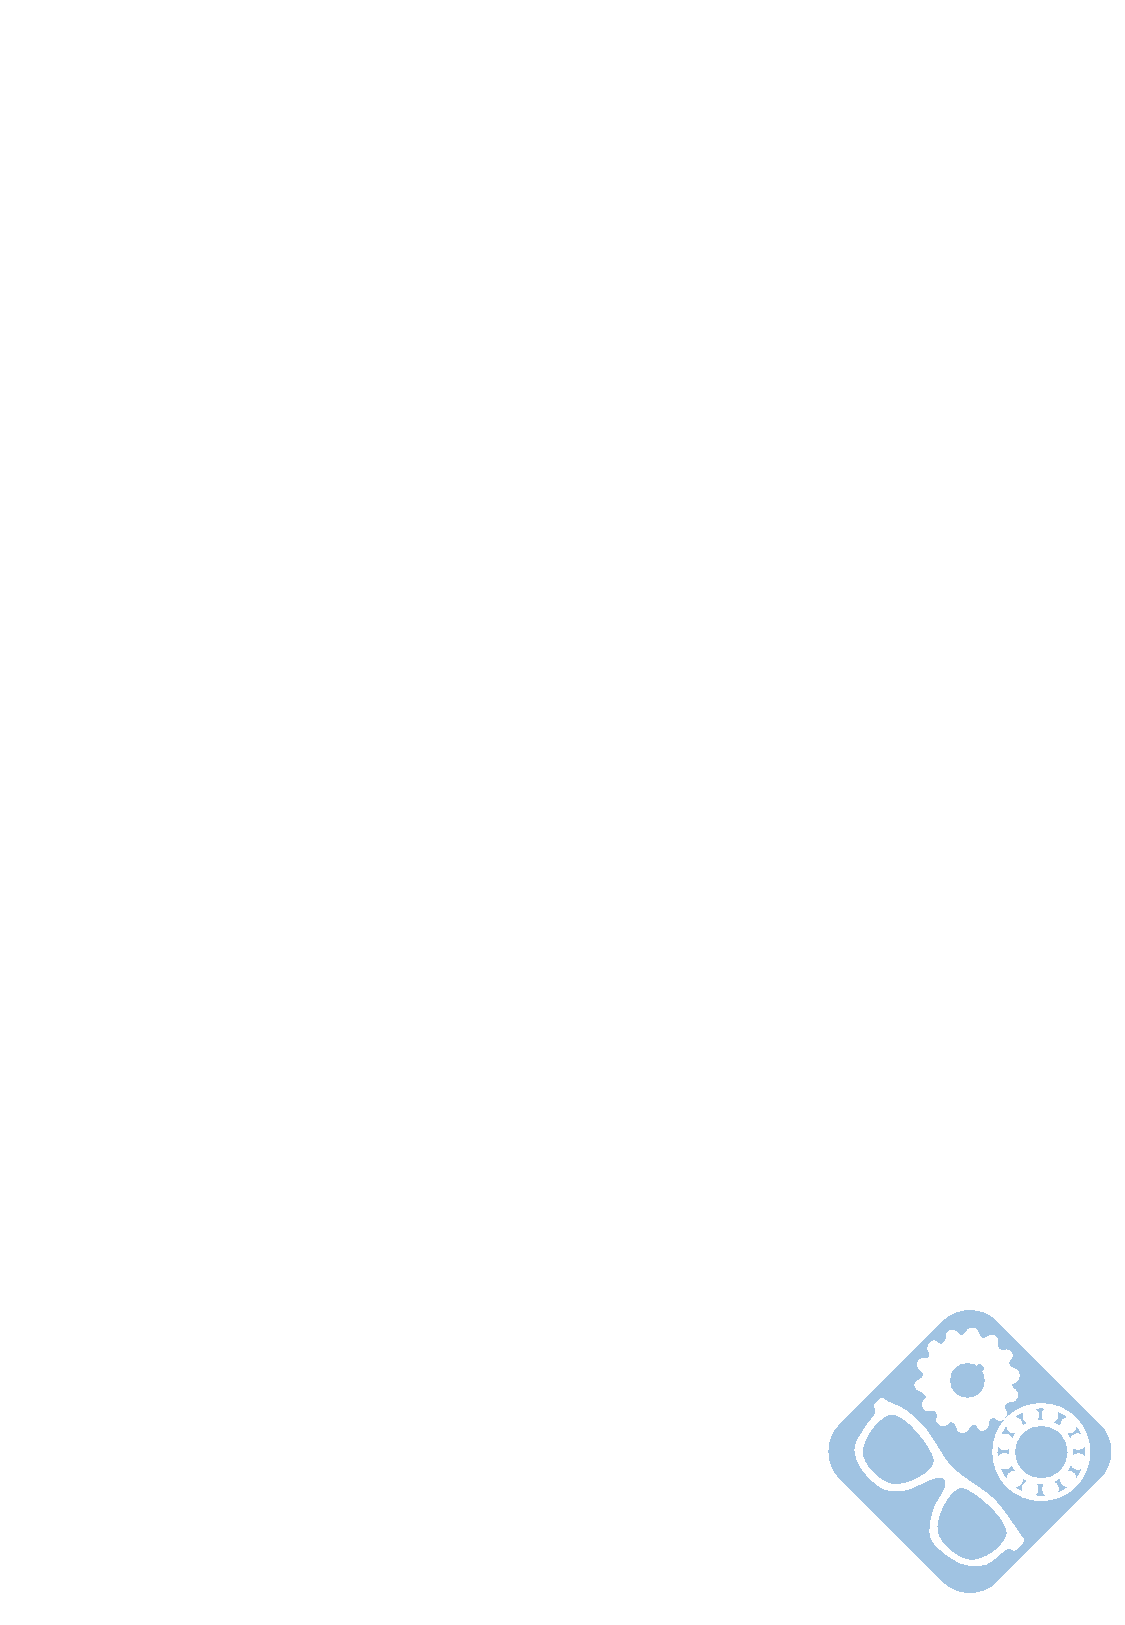
\includegraphics[width=\paperwidth,height=\paperheight,%
keepaspectratio]{../../img/fond4}%
\end{center}
\vfill
}}}

\begin{document}

\pagestyle{empty}

\vspace*{-3\baselineskip}

\AddToShipoutPicture*{\BackgroundPic}

\ifdef{\auteurdeux}{\begin{tabular}{>{\columncolor{gray!00}}m{.3\linewidth} m{.3\linewidth} >{\columncolor{gray!00}}m{.3\linewidth}}
Séquence : \sequence &  \multirow{3}{*}{\hspace{1cm}
\includegraphics[height=1.5cm]{../../img/logo}} &  \begin{flushright} \multirow{4}{*}{\hspace{1cm}
\includegraphics[height=4cm]{img/qrcode}}\end{flushright}\\
Document : \type\num \\
 \institute \\
 \auteurun\\
 \auteurdeux
\end{tabular}}{\begin{tabular}{>{\columncolor{gray!00}}m{.3\linewidth} m{.3\linewidth} >{\columncolor{gray!00}}m{.3\linewidth}}
Séquence : \sequence &  \multirow{3}{*}{\hspace{1cm}
\includegraphics[height=1.5cm]{../../img/logo}} &  \begin{flushright} \multirow{4}{*}{\hspace{1cm}
\includegraphics[height=4cm]{img/qrcode}}\end{flushright}\\
Document : \type\num \\
 \institute \\
 \auteurun
\end{tabular}}

\vspace{1cm}

\ifdef{\prive}{\begin{center}\colorbox{danger}{\Huge{Avec Correction}}\end{center}}{}

\begin{center}\huge{\nom}\end{center}

\vspace{2cm}

\ifdef{\imagedeux}{\begin{minipage}{0.49\linewidth}}{}
\begin{center}\includegraphics[height=5cm]{/home/renaud/Documents/Renaud/GitHub/django_education/systemes/\imageun}\end{center}
\ifdef{\imagedeux}{\end{minipage}\hfill
\begin{minipage}{0.49\linewidth}
\begin{center}\includegraphics[height=5cm]{/home/renaud/Documents/Renaud/GitHub/django_education/systemes/\imagedeux}\end{center}
\end{minipage}}{}

\vspace{5cm}


\begin{tabular}{p{.15\linewidth} >{\columncolor{white}}p{.8\linewidth}}
    \rowcolor{gray!20}
    Référence & S\sequence\ - \type\num \\
    Compétences & \competences \\
 	\rowcolor{gray!20}
    Description & \descrip \\
    Système & \systemes
  \end{tabular}

\newpage

\AddToShipoutPicture{\BackgroundPicdeux}

\pagestyle{normal}

\section{Fauteuil TopChair}
\subsection{Présentation du système}

\begin{wrapfigure}[8]{r}{6cm}
\vspace{-7mm}
\centering 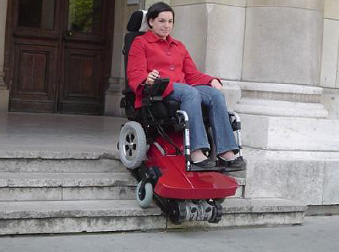
\includegraphics[width=0.9\linewidth]{img/img00}
\end{wrapfigure}
Plus d'autonomie pour plus de liberté! TopChair\textregistered{} offre aux personnes à mobilité réduite une nouvelle possibilité de se déplacer sans assistance à domicile, au travail ou en ville. Ce fauteuil roulant électrique est capable de franchir obstacles et marches sans nécessiter l'installation d'une structure fixe. Dans la plupart des cas, la présence d'un accompagnateur n'est pas nécessaire.

Une utilisation simple et confortable au quotidien: un seul bouton suffit pour passer du mode \og route \fg au mode \og escalier \fg.

TopChair\textregistered{} innove avec un double système de déplacement: sur ses roues en terrain plat et sur ses chenilles pour franchir des marches. Les chenilles sont en caoutchouc avec une armature très résistante en acier.

Un asservissement de position qui permet de maintenir l'orientation du siège constante quelle que soit l'inclinaison de la chaussée. Un micro-processeur à haute performance pour une sécurité optimale.

\subsubsection{Modes de fonctionnement}

On distingue 3 modes principaux de fonctionnement:
\begin{itemize}
 \item un mode \og route \fg{} où le fauteuil se comporte comme un fauteuil roulant classique, les roues arrières sont motrices, les changements de direction sont obtenus en faisant varier la vitesse de rotation des roues arrières gauche et droite, les deux roues folles à l'avant s'orientant dans la direction du virage,
 \item un mode \og chenille \fg{} (ou chemin) où la puissance est dirigée sur les chenilles (mode utile pour se sortir des situations difficiles), les changements de direction sont obtenus en pilotant séparément chaque chenille,
 \item un mode \og escalier \fg{} où le programme gère les actionneurs de façon à monter/descendre les escaliers.
\end{itemize}

\subsection{Etude escamotage des roues}

Nous allons nous intéresser à quelques éléments caractéristiques du fauteuil roulant TopChair\textregistered{}. Toutes les parties sont indépendantes et des résultats intermédiaires permettent de poursuivre l'étude.

Pour passer du mode \og route \fg{} aux deux autres modes, il est nécessaire d'escamoter les trains avant et arrière. L'escamotage des trains est assuré par deux vérins électriques (un pour l'avant, l'autre pour l'arrière). La masse du fauteuil et de son passager étant relativement importante, il est nécessaire, pour la sécurité du passager et la fiabilité du fauteuil, que la structure et les vérins soient correctement dimensionnés. Pour cela, nous allons:
\begin{itemize}
 \item valider la structure cinématique du mécanisme de basculement du train avant,
 \item concevoir la liaison entre le levier et l'arbre de basculement.
\end{itemize}

~\

\textbf{Hypothèses complémentaires}
\begin{itemize}
 \item Compte-tenu de la symétrie du fauteuil, l'étude sera réalisée dans ce plan de symétrie (mécanisme plan),
 \item Les mouvements sont suffisamment lents pour que l'on puisse réaliser une étude statique,
 \item Les chenilles sont fixes et solidaires du châssis,
 \item Pendant le mouvement, le siège reste horizontal ($\overrightarrow{x_7}=\overrightarrow{x_0}$),
 \item Les roues avant restent parallèles au châssis et dirigées vers l'avant ($\overrightarrow{x_6}=\overrightarrow{x_5}$).
\end{itemize}

\subsection{Étude de la commande des vérins du siège}

Objectif: vérifier l'aptitude de la fonction \og distribuer \fg à commander dans les deux sens à vitesse variable le moteur à courant continu d'inclinaison.

Cahier des charges(extrait):
\begin{itemize}
 \item la vitesse de déplacement de la tige du vérin doit varier de $0$ à $30 mm.s^-1$, dans les deux sens.
\end{itemize}

Si on veut assurer un confort maximal du passager, les mouvements du siège doivent se faire sans à-coups.Pour cela, il est nécessaire de pouvoir faire varier la vitesse des moteurs. Le schéma de commande des vérins électriques d'inclinaison du siège et de basculement du train avant et du train arrière est fourni en annexe A-11). Étude de la commande du moteur du vérin. Soit la structure suivante (figure 5 page suivante), extraite du schéma de la commande du vérin d'inclinaison (partie centrale du schéma en annexe A-11), dans laquelle on trouve les signaux de commande \og Incliner siège \fg et \og Redresser siège \fg.

\begin{center}
 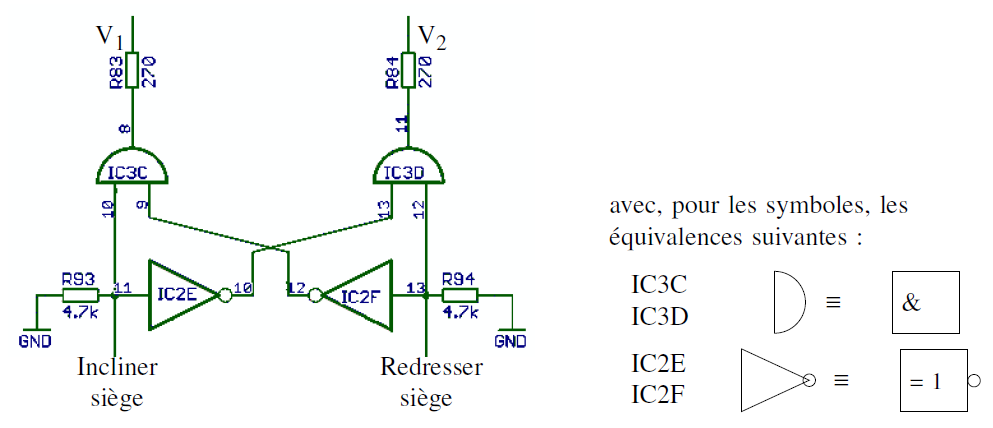
\includegraphics[width=0.8\linewidth]{img/img01}
\end{center}

\paragraph{Question 1:} Étude du circuit de commande
\begin{enumerate}
 \item Justifier que le niveau logique à l'entrée de IC2E est bas (niveau logique 0) lorsque le signal \og Incliner siège \fg est en haute impédance (\og z \fg dans la table de vérité). En déduire la fonction des résistances R93 et R94,
 \item Compléter sur la table de vérité de la structure,
 \item Préciser l'utilité d'une telle structure.
\end{enumerate}

~\

\begin{center}
\begin{tabular}{|c|c|c|c|}
\hline
Incliner & Redresser & $v_1$ & $v_2$ \\
\hline
0 & 0 &  &  \\
\hline
0 & 1 &  &  \\
\hline
1 & 0 &  &  \\
\hline
1 & 1 &  &  \\
\hline
z & z &  &  \\
\hline
\end{tabular}
\end{center}

~\

\textbf{Étude de la structure de distribution d'énergie au moteur du vérin.}

Soit le schéma partiel suivant et le schéma équivalent. Nous supposerons dans cette partie que le point A du schéma partiel est relié à la masse (GND 0V). 

\paragraph{Question 2:} Donner le nom de la structure réalisée sur le schéma réel de commande du moteur (figure 6(a)) et modélisée sur le schéma équivalent.

\paragraph{Question 3:} À partir du schéma équivalent, indiquer les interrupteurs à commander pour permettre la rotation du moteur dans le sens horaire ($u_{moteur}>0$) et dans le sens anti-horaire.

\paragraph{Question 4:} Sachant que les entrées $V_1$ et $V_2$ du schéma de commande peuvent prendre les niveaux logiques 0 ou 1 soit 0V ou 5V, donner les niveaux logiques de $V_1$ et $V_2$ permettant une tension positive aux bornes du moteur ($u_{moteur}>0$) et une tension négative aux bornes du moteur ($u_{moteur}<0$). Justifier votre réponse en précisant le rôle de Q3 et Q4.

\begin{center}
 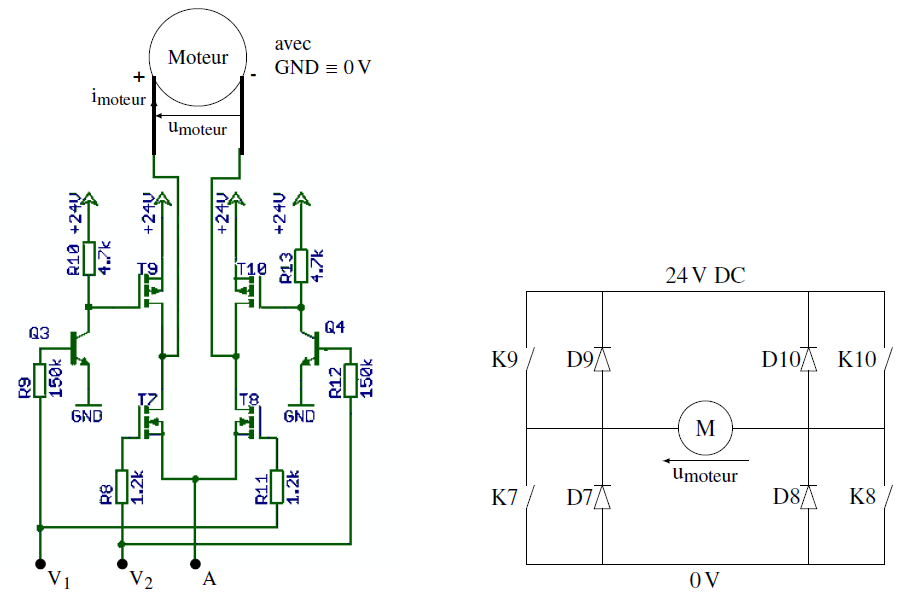
\includegraphics[width=0.8\linewidth]{img/img02}
\end{center}

Le document réponse suivant présente l'évolution des deux tensions $V_1$ et $V_2$ pour $\alpha>0,5$ et $\alpha<0,5$. On admet les hypothèses suivantes:
\begin{itemize}
 \item la structure fonctionne en régime moteur P>0,
 \item à $t=0$, le régime est établi en fonctionnement moteur,
 \item les transistors sont parfaits et la résistance d'induit $r$ du moteur est négligeable,
 \item si $\alpha>0,5$ on supposera que $i_{moteur}>0$ à $t=0$ et si $\alpha<0,5$ alors $i_{moteur}<0$ à $t=0$,
 \item la constante de temps du moteur étant très grande devant celle du hacheur, le sens de rotation du moteur dépend de la valeur moyenne de la tension à ses bornes.
\end{itemize}

\paragraph{Question 5:} Étude de $u_{moteur}$ (répondre sur le digramme suivant).
\begin{enumerate}
 \item Compléter le chronogramme de la tension $u_{moteur}$ en fonction des chronogrammes de $V_1$ et $V_2$.
 \item Calculer la valeur moyenne $U_{moy}$ de $u_{moteur}$ en fonction de $Vcc$ et de $\alpha(Vcc=24V)$.
 \item Tracer l'allure de $U_{moyen}$ fonction de $\alpha$ et préciser le sens de rotation sur la ligne \og sens de rotation \fg du chronogramme sachant que, pour $U_{moy}>0$, le moteur tourne dans le sens horaire.
\end{enumerate}

Les signaux \og Incliner Siège \fg et \og Redresser Siège \fg émis par le microcontrôleur ont un rapport cyclique variable ($0<\alpha<1$).

\paragraph{Question 6:} Nommer ce type de commande et conclure sur la capacité de la fonction \og distribuer \fg à obtenir une vitesse variable dans les deux sens du siège.

\begin{center}
 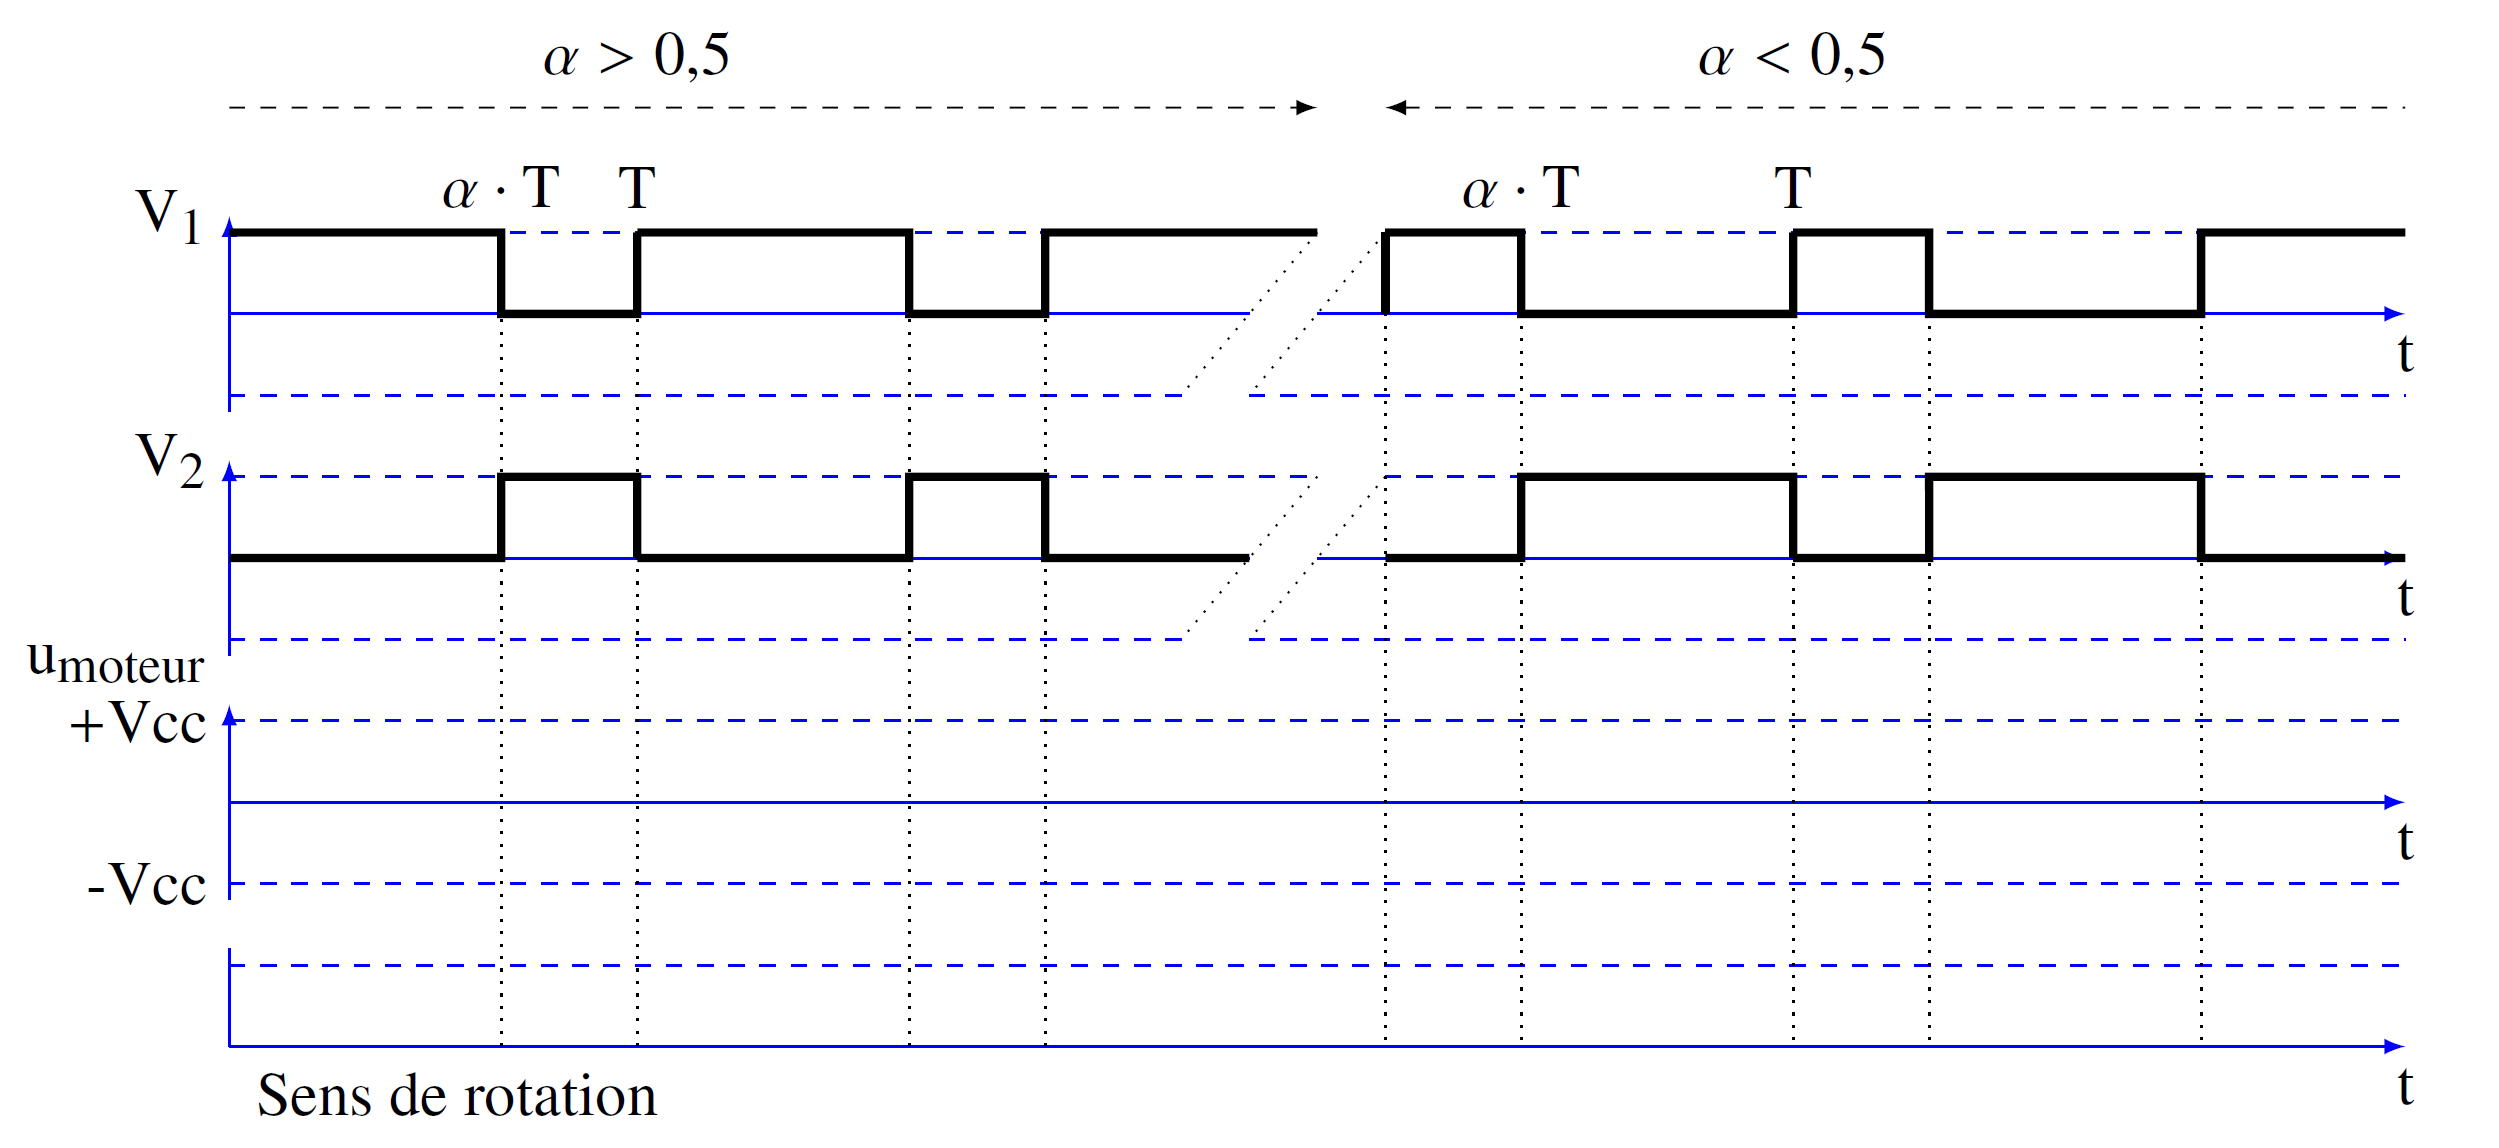
\includegraphics[width=0.9\linewidth]{img/doc_rep_chair}
\end{center}

Annexe sur les MOSFET

\begin{center}
 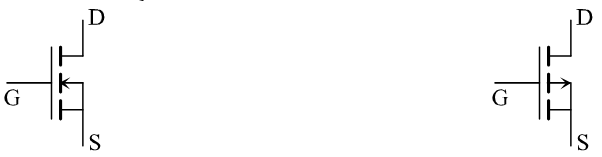
\includegraphics[width=0.7\linewidth]{img/img03}
\end{center}

T7 et T8 : Transistor MOSFET à canal N \hfill T9 et T10 : Transistor MOSFET à canal P

Les transistors T7 et T8 sont passants quand leur tension $v_{GS}>0$ et bloqués quand $v_{GS}=0$.
Les transistors T9 et T10 sont passants quand leur tension $v_{GS}=0$ et bloqués quand $v_{GS}>0$.

\newpage

\section{Système EOS}

Basé sur les travaux de Georges Charpak, prix Nobel de Physique 1992, EOS est un système d'imagerie
révolutionnaire commercialisé par la société EOS imaging depuis 2007. Il permet l'acquisition simultanée de
radiographies de face et de profil du corps entier (ou d'une zone anatomique localisée) avec une réduction de la
dose de rayons X de l'ordre de 90\% par rapport à un système radiographique conventionnel ou un scanner. Une
des originalités du système EOS est que le patient peut prendre place dans diverses positions correspondant
aux situations de la vie courante, ce qui permet d'obtenir des images de son corps
\og en charge \fg et donc une visualisation plus précise d'éventuelles pathologies (scoliose, trouble de la statique...).

\begin{figure}[!h]
 \centering 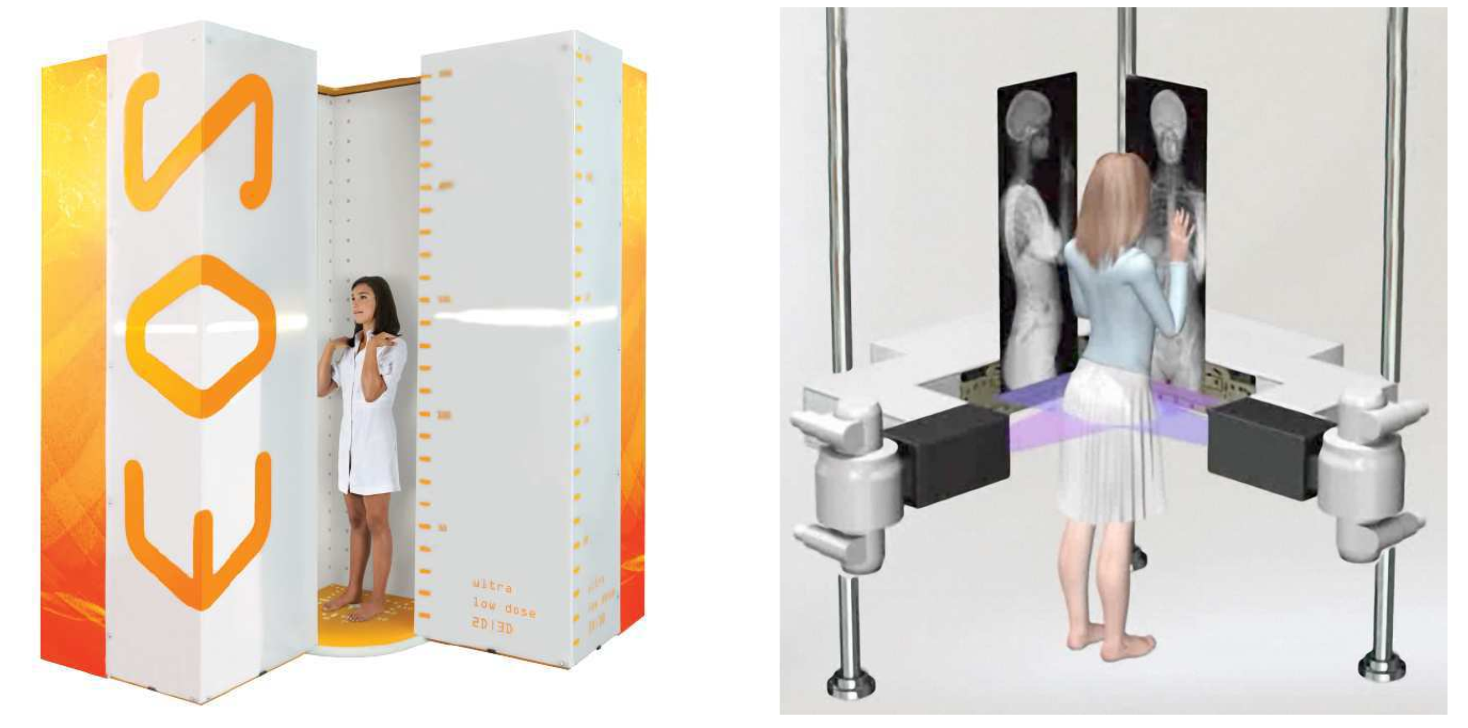
\includegraphics[width=0.8\linewidth]{img/td02_01}
 \caption{Vues extérieure et intérieure du système}
 \label{td02_01}
\end{figure}

\begin{figure}[!h]
 \centering 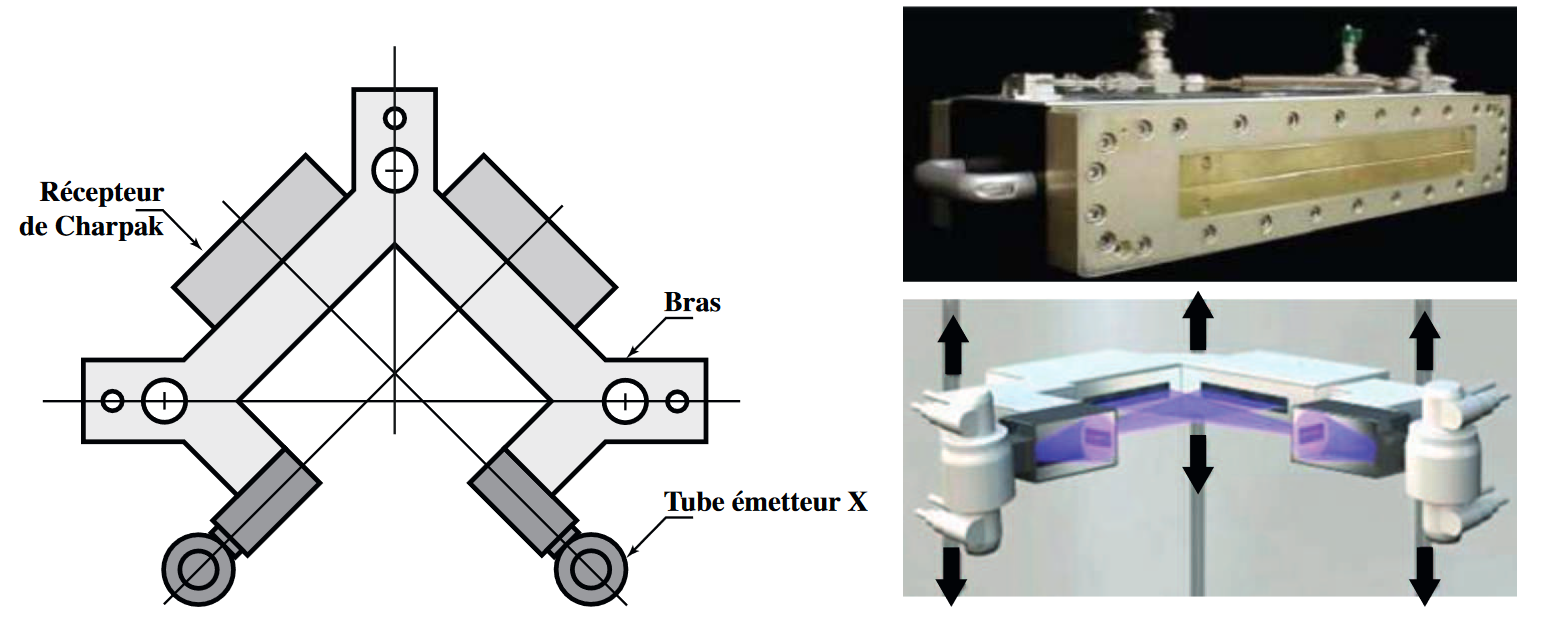
\includegraphics[width=0.8\linewidth]{img/td02_02}
 \caption{A gauche : bras mobile vue de dessus. En haut à droite : un des deux détecteurs de Charpak. En bas à droite : émission et réception des rayons}
 \label{td02_02}
\end{figure}

La figure \ref{td02_01} présente une vue extérieure et une vue intérieure du système. On peut notamment voir une
schématisation du mécanisme interne, constitué d'un bras mobile, guidé par rapport au bâti par trois colonnes
verticales. Comme le montre la figure \ref{td02_02}, le bras supporte deux chaînes d'acquisition, chacune d'entre elles étant composée d'un tube à rayons X et d'un détecteur. Les tubes émettent des rayons X en pinceaux très fins qui sont ensuite recueillis par les deux détecteurs issus de la technologie ayant valu le prix Nobel de Physique à Georges Charpak en 1992.

Durant un balayage vertical de quelques secondes, les deux chaînes permettent de faire l'acquisition simultanée d'une image de face et d'une de profil du corps entier ou d'une zone anatomique choisie.

A partir de ces images, un logiciel dédié permet de réaliser une modélisation tridimensionnelle du squelette du patient (cf. figure \ref{td02_03}) qui sera utilisée à des fins thérapeutiques.

\begin{figure}[!h]
 \centering 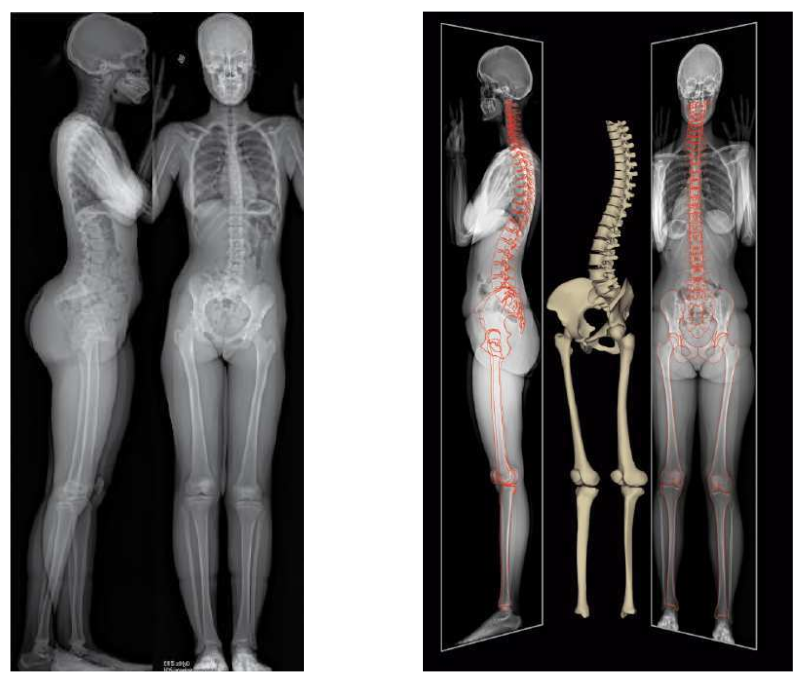
\includegraphics[width=0.8\linewidth]{img/td02_03}
 \caption{Exemple d'images acquises et reconstruction du squelette du patient}
 \label{td02_03}
\end{figure}

Afin de présenter les caractéristiques principales du système, un diagramme de contexte est donné sur la
figure \ref{td02_04}, ainsi qu'un diagramme partiel des exigences sur la figure \ref{td02_05}. Les principaux éléments du système EOS sont représentés sur le diagramme de définition de blocs de la Figure \ref{td02_06}. Les valeurs numériques associées aux différents critères seront introduites au fur et à mesure des besoins dans la suite du sujet.

\begin{figure}[!h]
 \centering 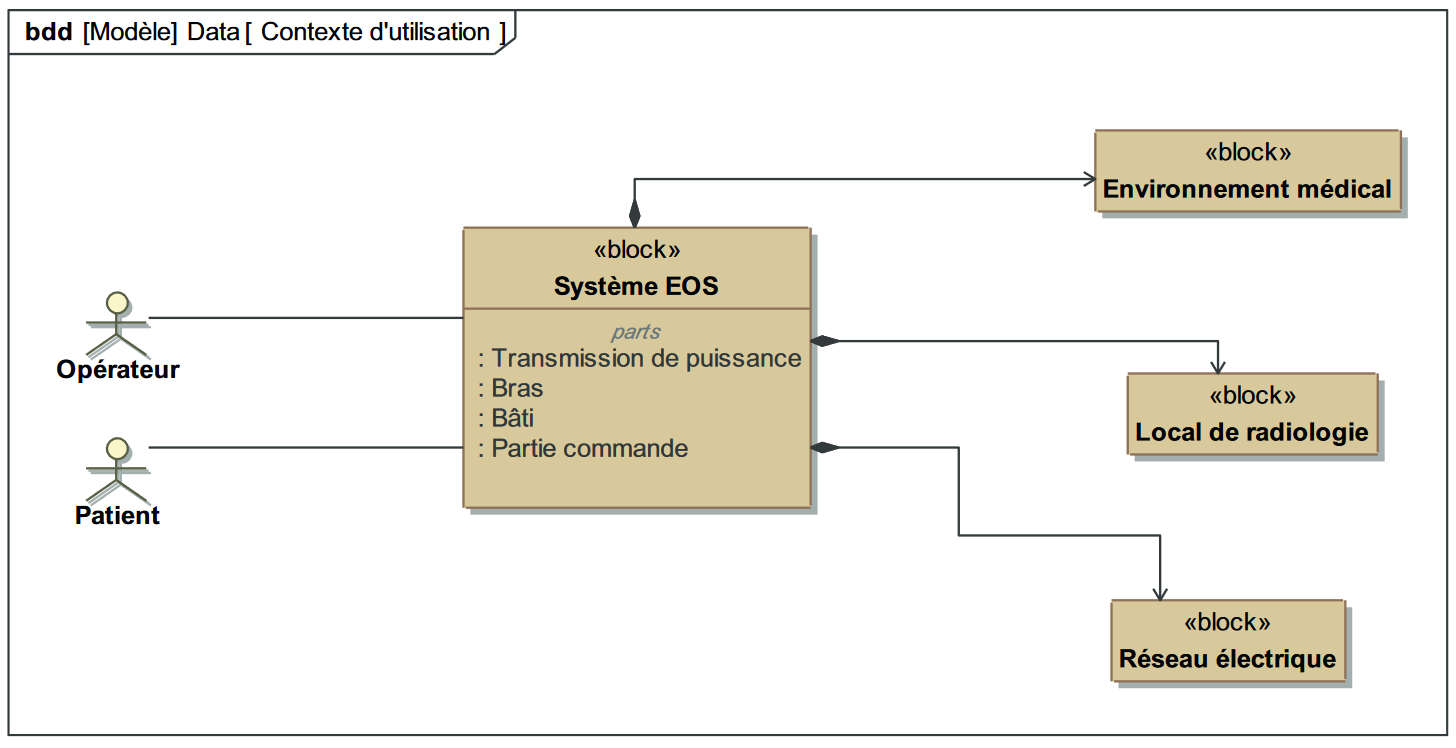
\includegraphics[width=0.8\linewidth]{img/td02_04}
 \caption{Diagramme de contexte du système EOS}
 \label{td02_04}
\end{figure}

\begin{figure}[!h]
 \centering 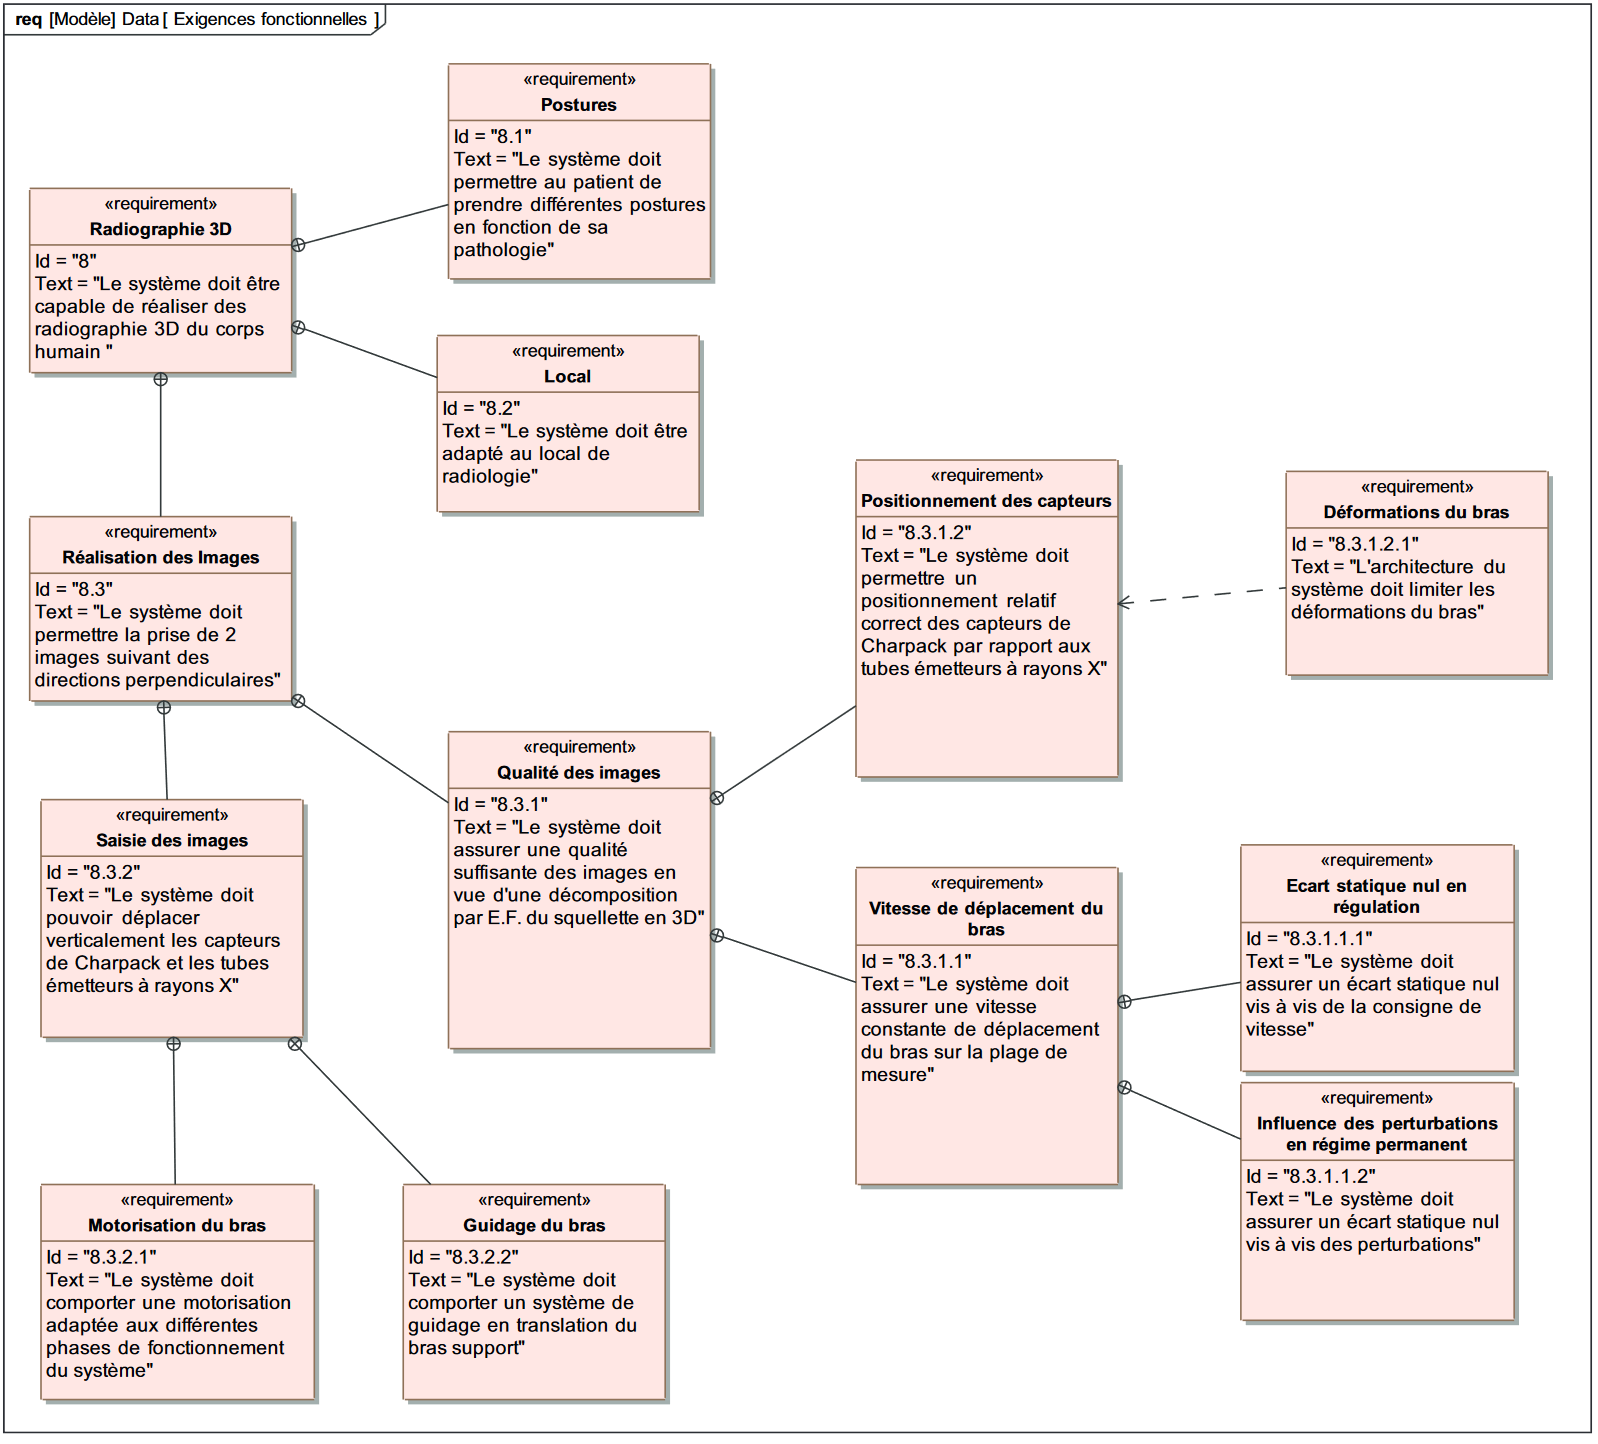
\includegraphics[width=0.8\linewidth]{img/td02_05}
 \caption{Diagramme partiel des exigences du système EOS}
 \label{td02_05}
\end{figure}

\begin{figure}[!h]
 \centering 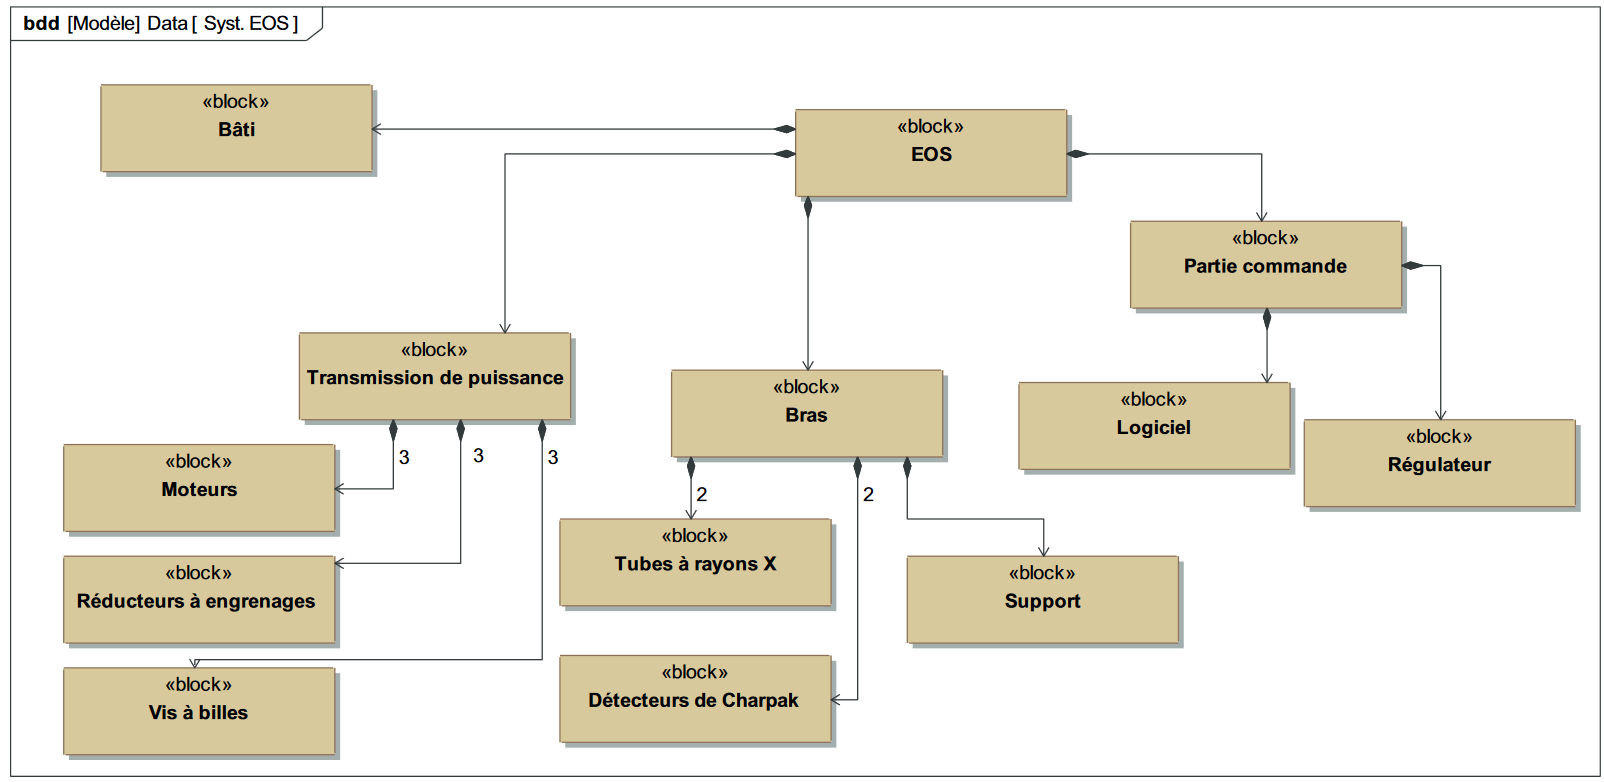
\includegraphics[width=0.8\linewidth]{img/td02_06}
 \caption{Diagramme de définition de blocs}
 \label{td02_06}
\end{figure}

\newpage

\subsection{Détermination de l'architecture du pré-actionneur électrique des moteurs à courant continu}

On considère que les 3 moteurs ainsi que les 3 circuits électriques sont identiques et que ces derniers sont
soumis à la même tension d'alimentation constante $U_{alim}$. Afin de faire varier la tension d'alimentation d'un moteur, on utilise un hacheur, placé en amont de chaque moteur. On se propose ici de déterminer la structure du hacheur compatible avec les éventuels différents modes de fonctionnement des moteurs lors d'un scan.

\subsubsection{Analyse de la pertinence d'un hacheur simple série}

On considère dans un premier temps un hacheur simple série (cf. figure \ref{td02_04}) constitué d'un interrupteur
commandé de type \og Transistor bipolaire à grille isolée (IGBT) \fg, de fréquence de découpage très grande par
rapport au temps caractéristique électrique du circuit, et d'une diode. L'interrupteur $K_1$ et la diode D sont supposés parfaits.

\begin{figure}[!h]
 \centering 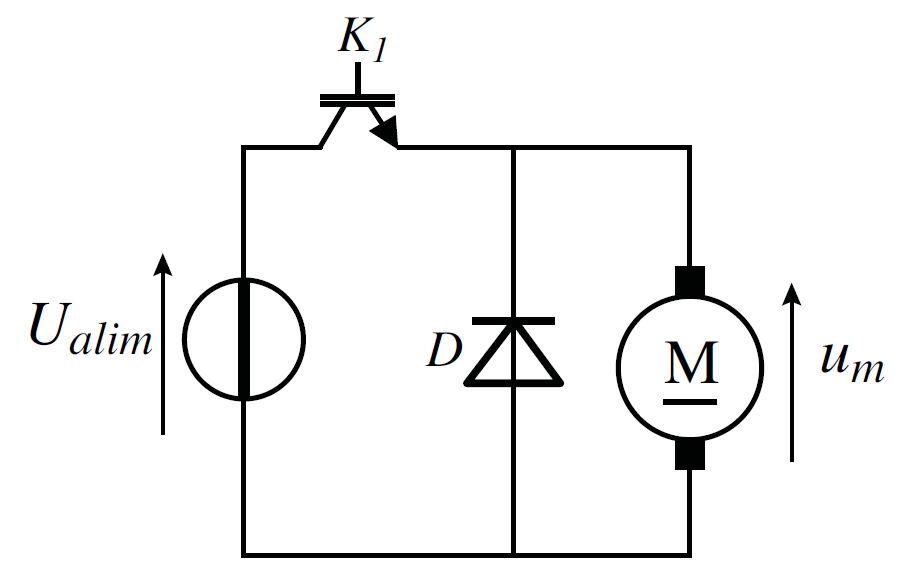
\includegraphics[width=0.8\linewidth]{img/td02_07}
 \caption{Schéma électrique de l'architecture simplifiée d'un hacheur simple série}
 \label{td02_07}
\end{figure}

\paragraph{Question 1:}

En considérant la phase de montée à vitesse constante, préciser sur la figure suivante en couleur les mailles dans lesquelles le courant circule lorsque le transistor est bloqué (rouge) ou passant (bleu). Ce type de hacheur permet-il les deux sens de courant dans le moteur (expliquer en trois lignes maximum). Préciser alors sur la figure suivante le(s) quadrant(s) dans le(s)quel(s) le moteur à courant continu peut fonctionner avec ce hacheur.

\begin{center}
 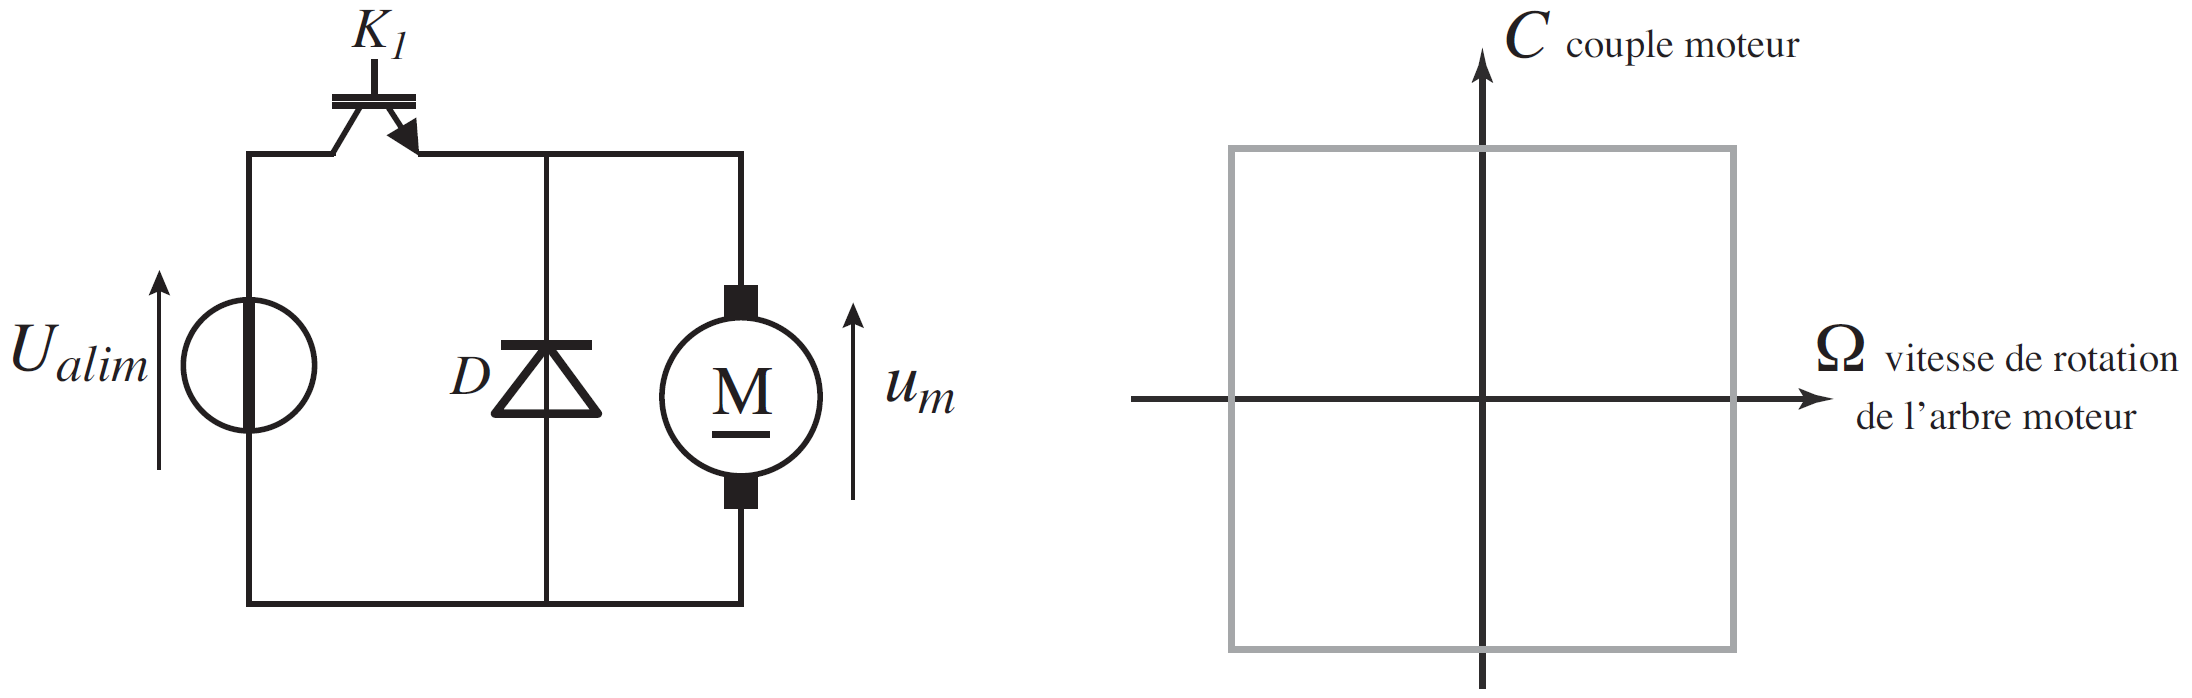
\includegraphics[width=0.8\linewidth]{img/td02_10}
\end{center}

On considère maintenant la phase de descente. Lors de cette phase, les moteurs doivent tourner dans le
sens inverse de celui de la phase de montée.

\paragraph{Question 2:}

Le hacheur proposé permet-il ces deux modes de fonctionnement (expliquer en trois lignes maximum) ?

\subsubsection{Analyse de la pertinence d'un hacheur réversible en tension}

En considère maintenant un hacheur réversible en tension dont le schéma d'une structure simplifiée est
donné sur la figure \ref{td02_08}. Sur une période de découpage T, les interrupteurs sont pilotés de la manière suivante ($\alpha$ étant le rapport cyclique compris entre 0 et 1) :
\begin{itemize}
 \item sur l'intervalle $[0,\alpha T[$ les interrupteurs $K_1$ sont passants,
 \item sur l'intervalle $[\alpha T , T[$ les interrupteurs $K_1$ sont bloqués.
\end{itemize}

\begin{figure}[!h]
 \centering 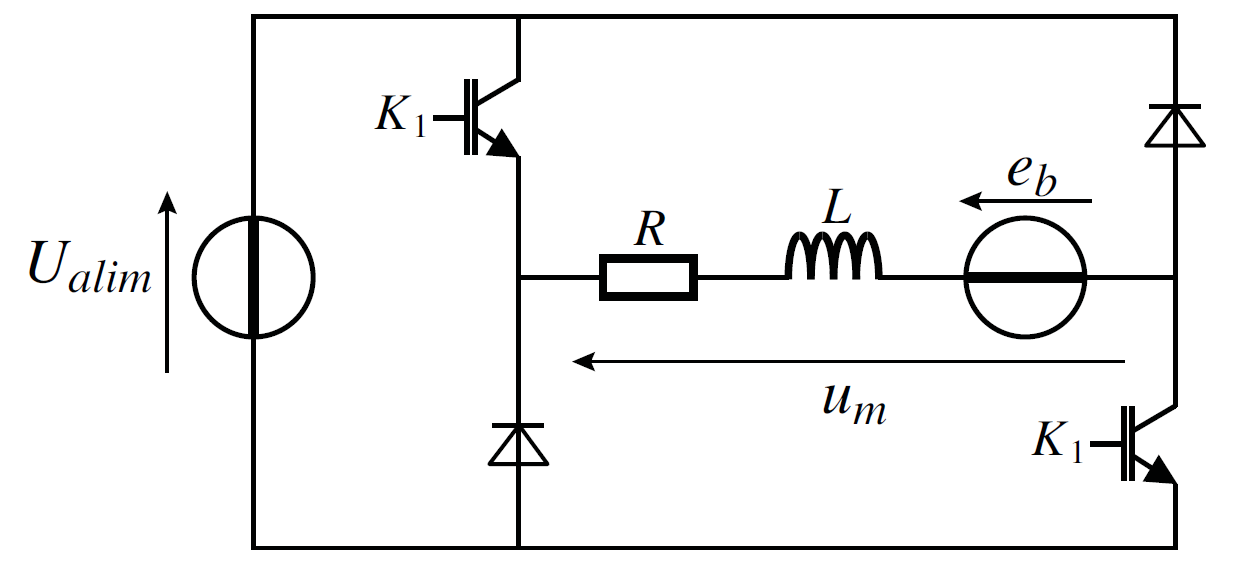
\includegraphics[width=0.8\linewidth]{img/td02_08}
 \caption{Schéma électrique de l'architecture simplifiée d'un hacheur réversible en tension}
 \label{td02_08}
\end{figure}

\paragraph{Question 3:}

En considérant la tension $U_{alim}$ constante, représenter sur le chronogramme suivant le graphe de
$u_m(t)$ sur une période $T$. Déterminer l'expression de la valeur moyenne de $u_m(t)$ sur une période $T$ (notée $<u_m>$) en fonction de $U_{alim}$ et de $\alpha$. Quelle est la plage de variation de $<u_m>$ ? Cette plage est-elle compatible avec les deux sens de rotation ?

\begin{center}
 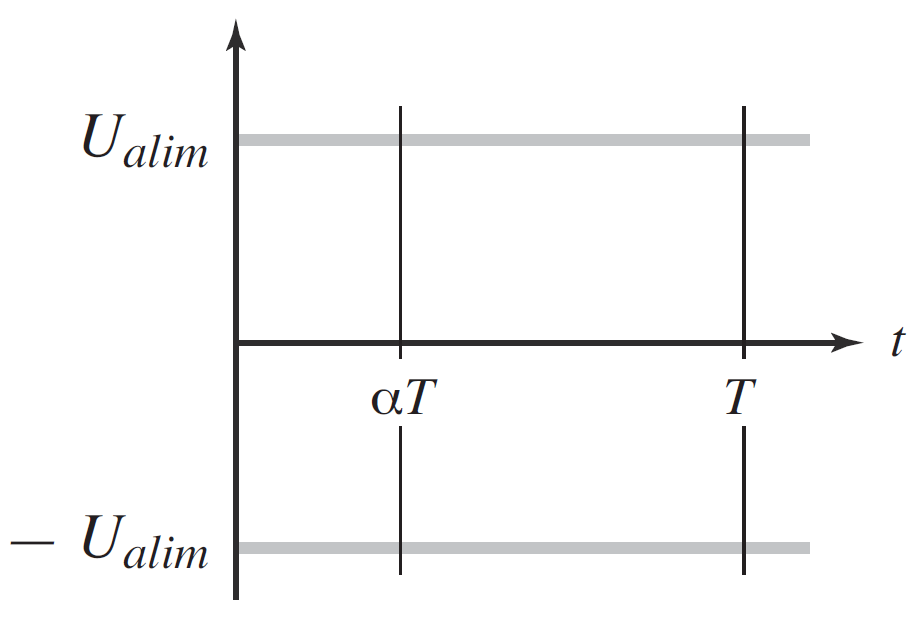
\includegraphics[width=0.8\linewidth]{img/td02_11}
\end{center}

\paragraph{Question 4:}

Préciser sur la figure suivante le(s) quadrant(s) dans le(s)quel(s) le moteur à courant continu peut fonctionner avec ce hacheur. Ce hacheur est-il compatible avec tous les modes de fonctionnements abordés (en phase de montée et en phase de descente) ?

\begin{center}
 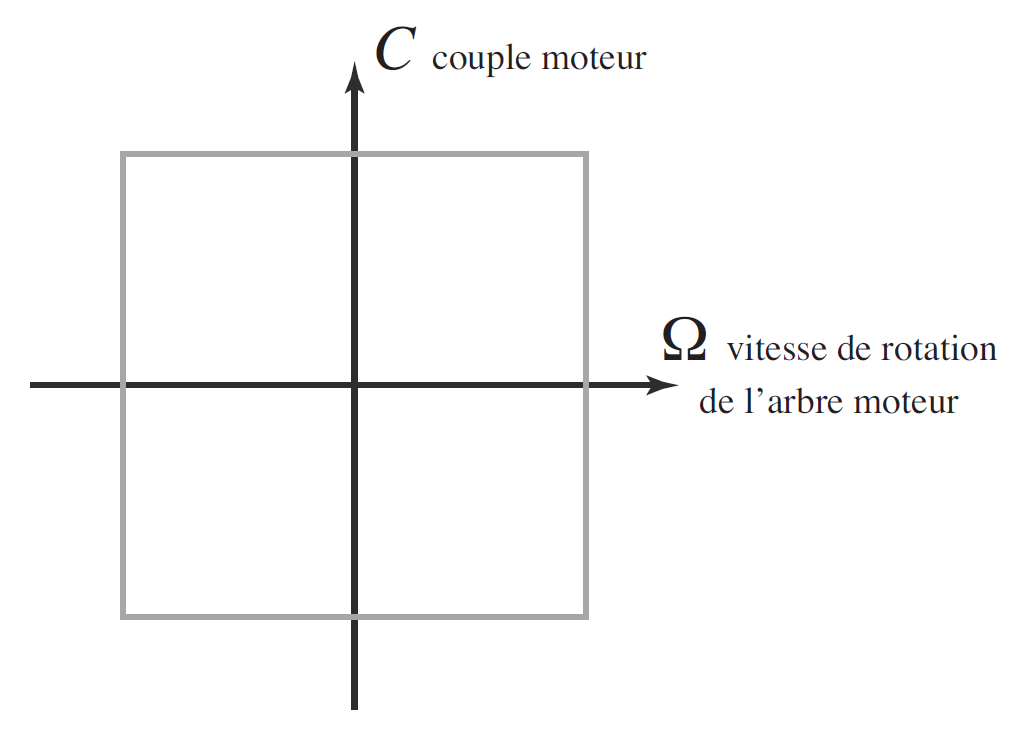
\includegraphics[width=0.8\linewidth]{img/td02_12}
\end{center}


\subsubsection{Analyse de l'influence du hacheur sur l'évolution du courant dans le circuit}

Quels que soient les résultats obtenus précédemment, on considère pour la suite le hacheur réversible en
tension. Dans le cas ù cette architecture ne serait pas compatible avec tous les modes de fonctionnement
des moteurs, un hacheur réversible en courant et tension serait adopté. Ces deux architectures ayant le même
impact sur la forme du courant dans le circuit au cours du temps, on se contente ici d'analyser le comportement
du circuit avec un hacheur réversible en tension.

On considère la phase de montée à vitesse constante et le rendement de la chaîne de transmission de
puissance est pris égal à 1.

On donne le bilan des puissances suivant:

$3\cdot C_m\cdot\omega_m=M\cdot g\cdot V$

Avec:
\begin{itemize}
 \item Pas de la vis (mm): $p_v=10$,
 \item Rapport de réduction : $N=5$,
 \item Masse(kg): $M=400$,
 \item Constante de couple (N.m/A): $K_i=0,12$,
 \item Résistance ($\Omega$): $R=2$,
 \item Tension d'alimentation (V): $U_{alim}=48$.
\end{itemize}

\paragraph{Question 5:}

Déterminer la valeur du courant $i_m$ traversant chaque moteur.

On cherche maintenant à déterminer l'évolution du courant pendant cette phase sur une période T. Sur l'intervalle de temps $[0,\alpha T[$, les transistors $K_1$ sont passants (Figure 16). L'intensité du courant à $t = 0$, est
notée $i_0$.

\paragraph{Question 6:}

Déterminer l'équation différentielle pilotant le comportement temporel de l'intensité du courant $i(t)$ traversant le moteur.

\paragraph{Question 7:}

Expliquer pourquoi $e_b(t)$ peut être considérée par hypothèse comme constante (on notera sa valeur $e_m$) puis, par la méthode de votre choix, déterminer l'expression de la fonction $i(t)$ en fonction de : $U_{alim}$, $e_m$, $R$, $i_0$ et une constante de temps $\tau_e=\frac{L}{R}$.

\paragraph{Question 8:}

On suppose que $T<<\tau_e$. En faisant un développement limité à l'ordre 1 de $i(t)$ au voisinage de zéro, déterminer $i(\alpha.T)$. Tracer sur la figure suivante l'allure du graphe de $i(t)$ sur une période complète $[0, T]$.

\begin{center}
 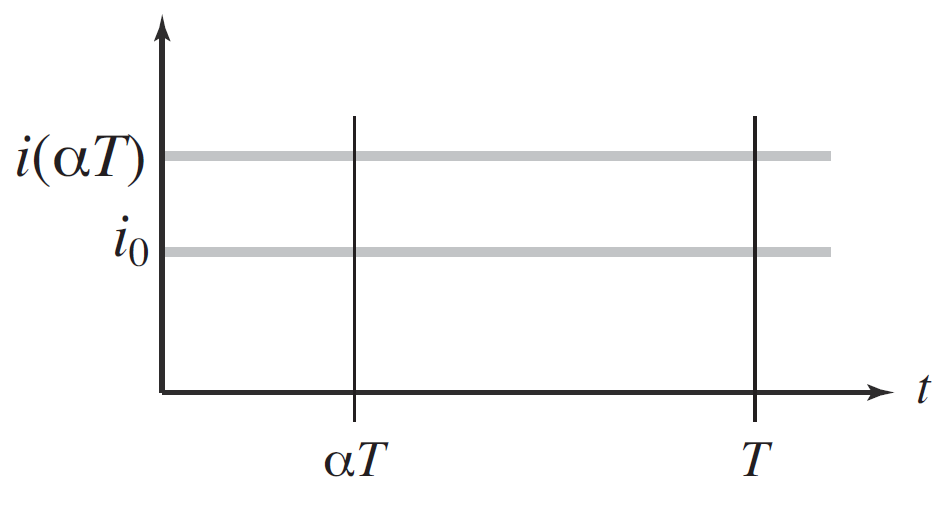
\includegraphics[width=0.8\linewidth]{img/td02_13}
\end{center}


\begin{figure}[!h]
 \centering 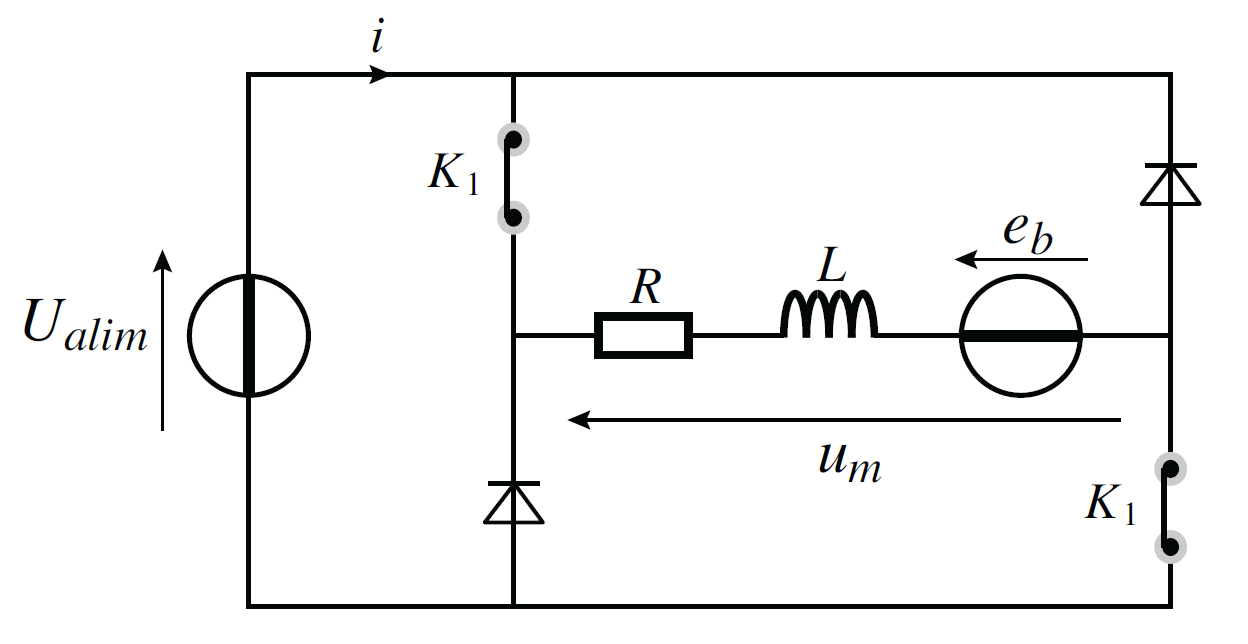
\includegraphics[width=0.8\linewidth]{img/td02_09}
 \caption{Schéma électrique de l'architecture simplifiée d'un hacheur réversible en tension, transistors passants}
 \label{td02_09}
\end{figure}

\paragraph{Question 9:}

En considérant toujours $T << \tau.e$, déterminer l'expression de l'augmentation de courant sur l'intervalle $[0, \alpha T[$:

$\Delta i =i(\alpha T)-i_0$  en fonction de $U_{alim}$, $e_m$, $R$, $\tau_e$ et $i_0$.

Afin que cette évolution de l'intensité du courant sur une période T ne perturbe pas le comportement
mécanique du moteur, on impose que $\Delta_i \simeq \frac{i_0}{100}$.

\paragraph{Question 10:}

En déduire une condition sur l'ordre de grandeur de $T$ par rapport à $\tau_e$. Dans la suite, on supposera que le hacheur choisi vérifie cette condition et par conséquent que les évolutions du courant sur une période T n'ont pas d'influence sur le comportement électromécanique de la chaîne de transmission de puissance. On prendra $e_m=36V$ pour l'application numérique.

\ifdef{\public}{\end{document}}

\newpage

\pagestyle{correction}

\section{Correction}

\paragraph{Question 1:} 

1. Les résistances (R93 et R94) permettent de mettre à 0 l'entrée des circuits logiques lorsque les signaux de pilotage sont en haute impédance.

2. Table de vérité du pilotage moteur :

\begin{center}
\begin{tabular}{|c|c|c|c|}
\hline
Incliner & Redresser & $v_1$ & $v_2$ \\
\hline
0 & 0 & 0 & 0 \\
\hline
0 & 1 & 0 & 1 \\
\hline
1 & 0 & 1 & 0 \\
\hline
1 & 1 & 0 & 0 \\
\hline
z & z & 0 & 0 \\
\hline
\end{tabular}
\end{center}

Équations logiques des sorties : \\
$v_1$=Incliner./Redresser \\
$v_2$=/Incliner.Redresser
 
3. Cela permet le verrouillage pour ne pas avoir tout mouvement lorsque l'inclinaison et le redressement sont demandés en même temps.

\paragraph{Question 2:} 
Pont en H (hacheur 4 quadrants).

\paragraph{Question 3:} 

Pour obtenir $u_{moteur}>0$, il faut commander les interrupteurs K8 et K9.\\
Pour obtenir $u_{moteur}<0$, il faut commander les interrupteurs K7 et K10.

\paragraph{Question 4:} 

Les résistances R9, R10 et le transistor Q3 permettent de réaliser une fonction NON. De même pour les résistances R12, R13 et le transistor Q4.

\begin{center}
\begin{tabular}{|c|c|c|}
\hline
$v_1$ & $v_2$ & Signe u moteur\\
\hline
1 & 0 & $u_{moteur}>0$ \\
\hline
0 & 1 & $u_{moteur}<0$ \\
\hline
\end{tabular}
\end{center}

\paragraph{Question 5:} 
1. Chronogrammes de la tension aux bornes du moteur :

\begin{center}
 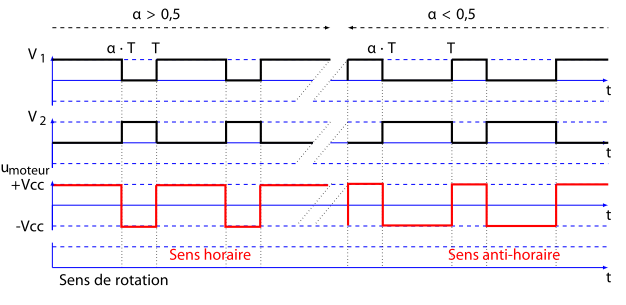
\includegraphics[width=0.7\linewidth]{img/img04}
\end{center}

2. Calcul de $<u_{moteur}$:

En utilisant la méthode des aires : $U_{moy}=\dfrac{\alpha.T.Vcc-(1-\alpha).T.Vcc}{T}$, $U_{moy}=^(2\alpha-1)Vcc$

3. Allure de $U_{moy}$:

\begin{center}
 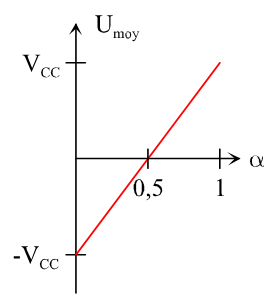
\includegraphics[width=0.3\linewidth]{img/img05}
\end{center}

\paragraph{Question 6:} 
Commande MLI (PWM). La fonction \og distribuer \fg est capable d'obtenir une vitesse variable dans les deux sens du siège.

\subsection{Système EOS}

\paragraph{Question 1:}

Le transistor IGBT et la diode sont des composants unidirectionnels en courant donc ce hacheur ne permet qu'un seul sens de courant dans le moteur.

\begin{center}
 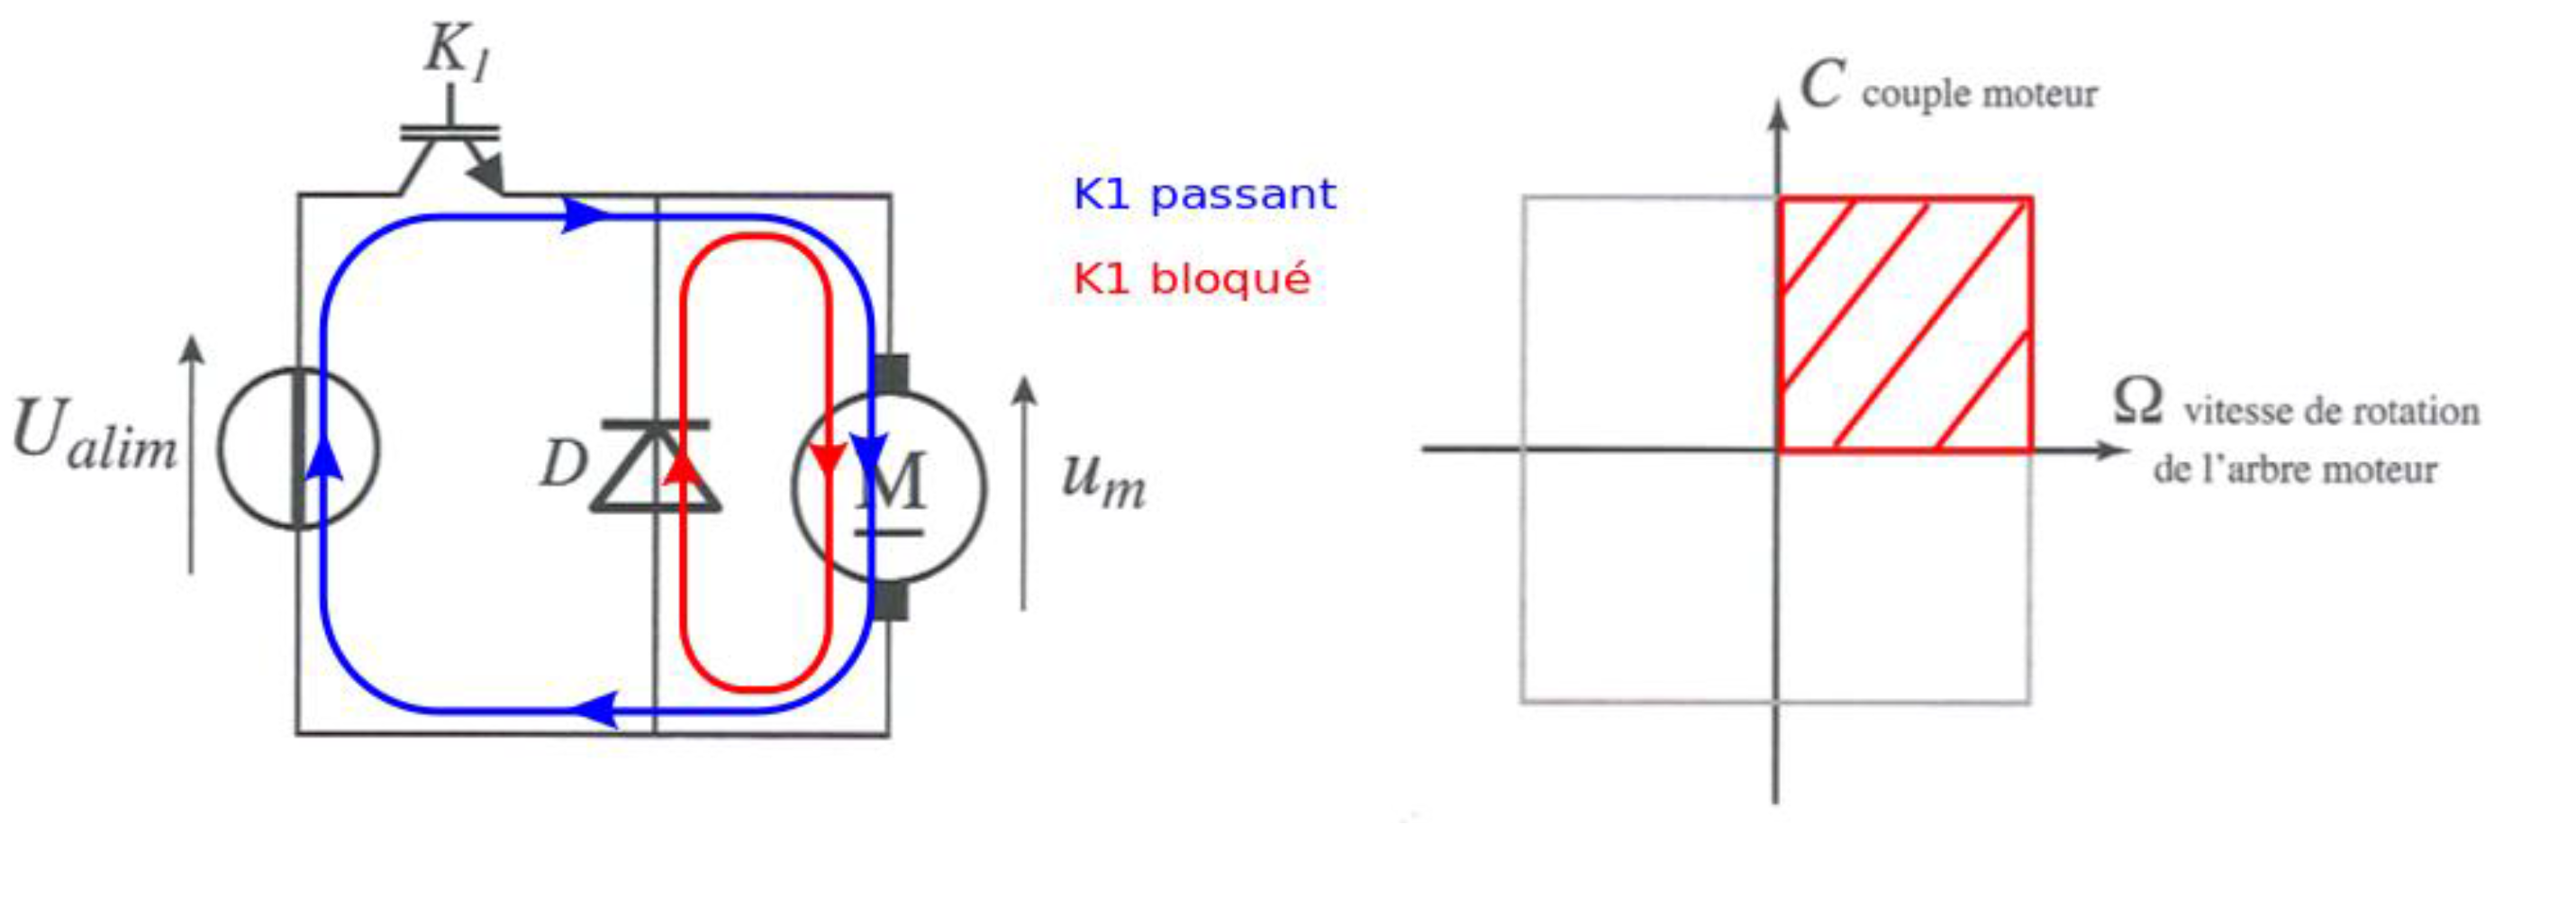
\includegraphics[width=0.3\linewidth]{img/td02_14}
\end{center}

\paragraph{Question 2:}

Le hacheur proposé est irréversible en tension et ne permet pas d'inverser la tension de
commande du moteur. Le moteur ne peut donc pas tourner dans le sens inverse.

\paragraph{Question 3:}

\begin{center}
 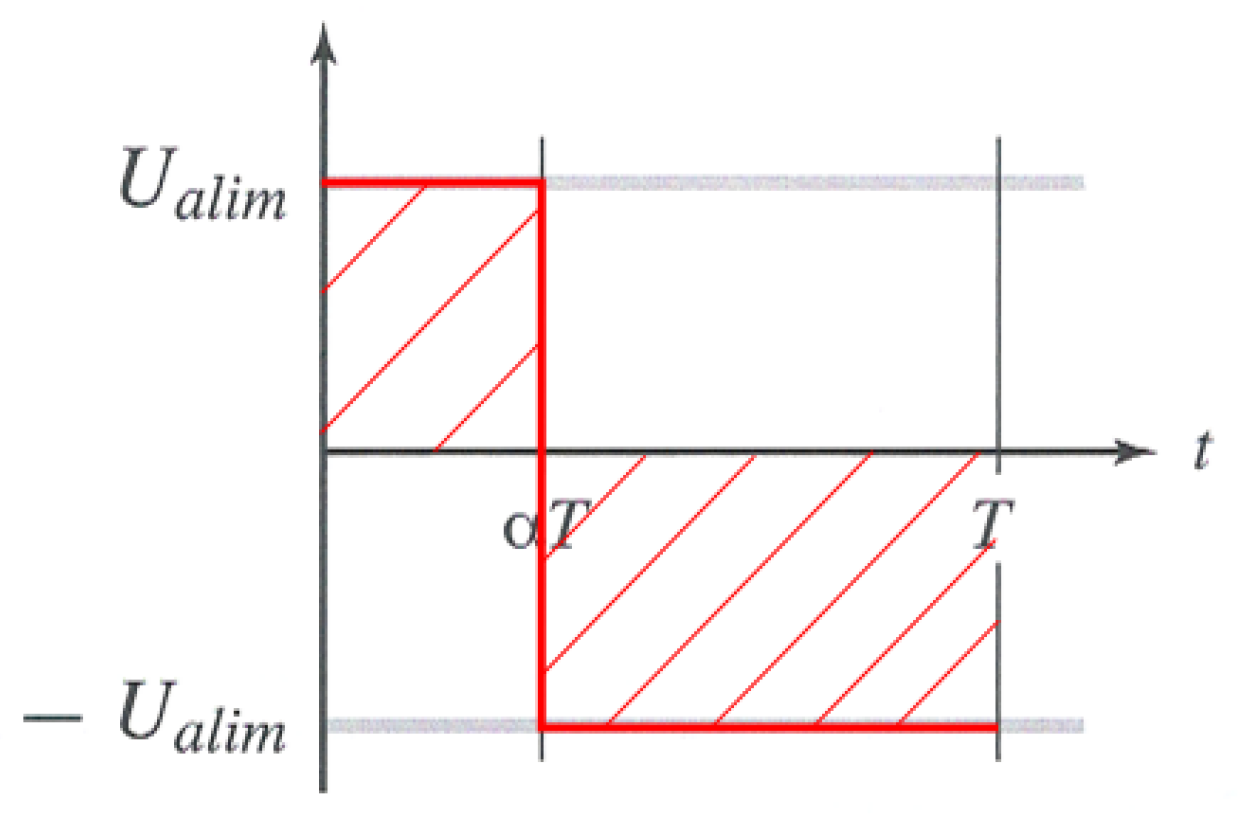
\includegraphics[width=0.6\linewidth]{img/td02_15}
\end{center}

$<u_m>=\frac{\alpha.T.U_{alim}-U_{alim}.(T-\alpha.T)}{T}=U_{alim}.(2.\alpha-1)$

Comme $\alpha\in[0,1]$, on a : $-U_{alim}<u_m<U_{alim}$

$<u_m>$ peut changer de signe, cette plage est donc compatible avec les deux sens de rotation.

\paragraph{Question 4:}

\begin{center}
 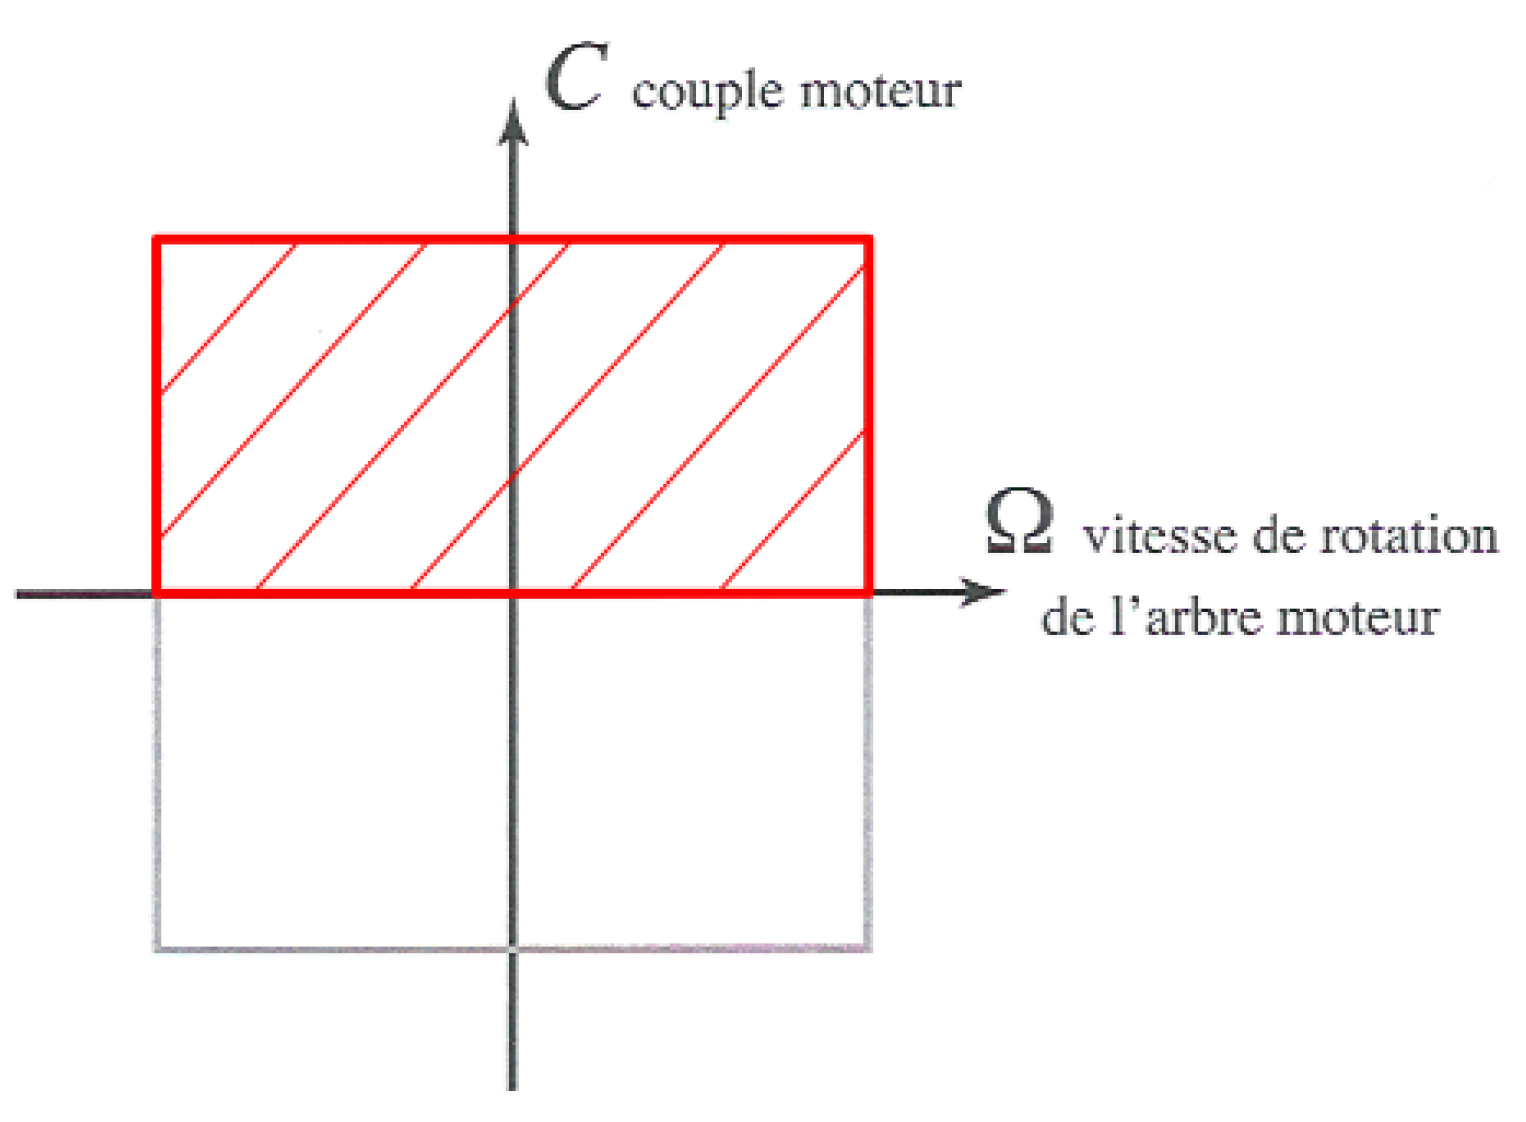
\includegraphics[width=0.3\linewidth]{img/td02_16}
\end{center}

Ce hacheur est réversible en tension et permet d'inverser le sens de rotation du moteur (montée et descente). Par contre, il ne permet de freiner le plateau pendant la phase de descente puisqu'il est irréversible en courant. 

\paragraph{Question 5:}

$3.C_m.\omega_m=M.g.V$, donc $3.K_i.i_m.\omega_m=M.g.\frac{p_v}{2.\pi}\frac{\omega_m}{N}$

Donc, $i_m=\frac{M.g.p_v}{6.\pi.N.K_i}\simeq 4A$

\paragraph{Question 6:}

$U_{alim}=e_b+R.i+L.\frac{di}{dt}$

\paragraph{Question 7:}

$\frac{di}{dt}=(\frac{U_{alim}-e_m}{R}-i).\frac{R}{L}$

Solution sans second membre: $i_g(t)=k.e^{-\frac{t}{\tau_e}}$, avec $\tau_e=\frac{L}{R}$

Solution particulière: $i_p(t)=\frac{U_{alim}-e_m}{R}$

$i(t)=\frac{U_{alim}-e_m}{R}.(1-e^{-\frac{t}{\tau_e}})+i_0.e^{-\frac{t}{\tau_e}}$

\paragraph{Question 8:}

En faisant un développement limité et en prenant t proche de 0, on obtient:

$i(t)=\frac{U_{alim}-e_m}{L}.t+i_0$

Et si $t=\alpha.T$, $i(\alpha.T)=\frac{U_{alim}-e_m}{L}.\alpha.T+i_0$.

\begin{center}
 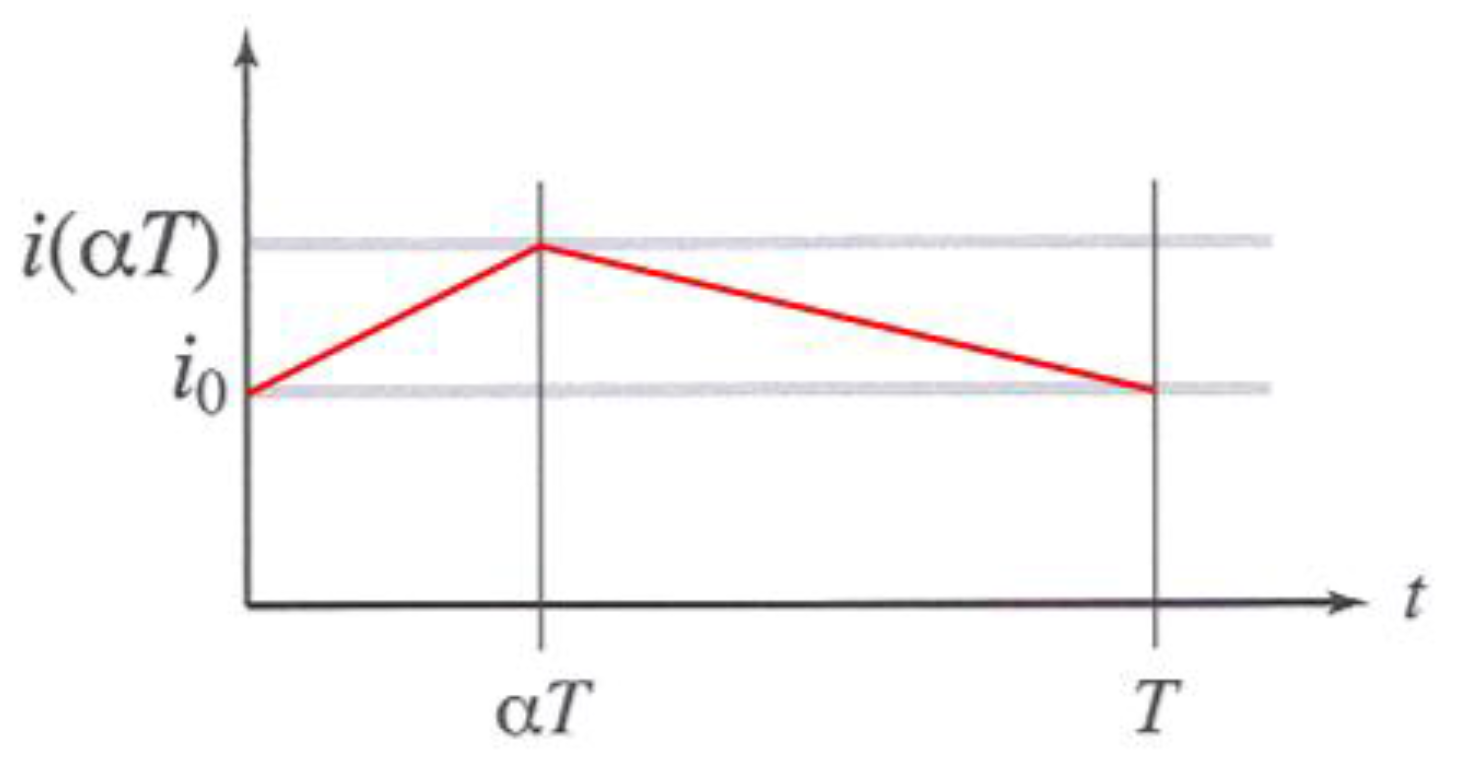
\includegraphics[width=0.3\linewidth]{img/td02_17}
\end{center}

\paragraph{Question 9:}

Toujours dans les mêmes conditions, on détermine l'augmentation de courant $\Delta_i$ défini par :

$\Delta_i=i(\alpha.T)-i_0=\frac{U_{alim}-e_m}{L}.\alpha.T$

\paragraph{Question 10:}

$\alpha \in [0,1]$, donc $\Delta_i<\frac{U_{alim}-e_m}{R}.\frac{T}{\tau_e}$

Afin de ne pas perturber le comportement mécanique du moteur, on impose : $\Delta_i\simeq\frac{i_0}{100}$.

On a donc: $\frac{T}{\tau_e}=\frac{R}{U_{alim}-e_m}.\frac{i_0}{100}$

Donc, $\frac{T}{\tau_e}\simeq\frac{2.0,04}{48-36}\simeq\frac{2}{3}.10^{-2}$

$\frac{T}{\tau_e}$ doit être de l'ordre de $\frac{1}{100}$.

\end{document}
